\chapter{Efficiency}
\label{sec:Rkst_efficiency}


The efficiency for each of the decay channels is calculated according to the formula
\begin{equation}
\varepsilon^{tot}=\varepsilon(geom)\varepsilon(reco|geom)\varepsilon(PID|reco)\varepsilon(trig|PID)\varepsilon(MVA|trig).
\end{equation}
In this expression the first term is the efficiency to have final state particles in the LHCb detector 
acceptance. The second term carries information on reconstruction and stripping efficiency
(we keep these together given that boundaries between them are completely artificial).
The third part corresponds to the efficiency of the PID requirements.
The fourth term handles the trigger efficiency for those events which are selected by the preselection process.
Finally, the latter term deals with the efficiency of the NN classifier.
Reconstruction, trigger and MVA efficiencies are evaluated on simulated data with the trigger efficiency
for $\Bz\to\Kstar\jpsi$ being cross-checked using the data-driven TISTOS method as described in Sec.~\ref{sec:Lb_trig_eff}.
The PID efficiency is calculated with a data-driven method as described in Sec.~\ref{sec:RKst_pid_eff}.

All absolute efficiencies for the muonic and electronic rare channels are separately listed in Tab.~\ref{tab:RKst_AbsEff}
for the central and high \qsq intervals and in Tab.~\ref{tab:AbsEff_jpsi} for the resonant channels.
However for the analysis itself only efficiencies relative to the resonant channels are used in order
to limit systematic uncertainties.
%($\varepsilon(\Bz\to\Kstar ee)/\varepsilon(\Bz\to\Kstar(\jpsi\to ee))$)/($\varepsilon(\Bz\to\Kstar \mumu)/\varepsilon(\Bz\to\Kstar(\jpsi\to \mumu))$).
%Systematic uncertainties for relative efficiencies take into account that some effects are correlated between two decays.
%In table \ref{tab:AbsEffs} are reported absolute efficiencies
%for the electron and muon channels in the \qsq bin $1 < q^2 < 6$ \gevgevcccc.

In Tab.~\ref{tab:RKst_AbsEff} are reported relative efficiencies between the rare and resonant channels,
$\varepsilon(\Bz\to\Kstar \ell^+\ell^-)/\varepsilon(\Bz\to\Kstar(\jpsi\to \ell^+\ell^-)$.
Finally, in Tab.~\ref{tab:double_rel_eff} are reported ratios of relative efficiencies
for the $ee$ and $\mu\mu$ channels, $(ee/(\jpsi \to ee))/(\mumu/(\jpsi\to \mumu))$.
%In particular the latter table contains the total double-relative
%efficiency, $\varepsilon_tot^{drel} = \pm $, which is used for the final result extraction.

\begin{table}
\centering
\begin{tabular}{|c|c|c|c|c|}
\hline Comp 			&  $\mu\mu$ 	& \multicolumn {3}{c|}{$ee$} \\ \hline
	&   &  L0Electron 	& L0Hadron 	& L0TIS \\ \hline
gen  & $ 0.1598  \pm  0.0005 $ & \multicolumn{3}{c|}{$ 0.1589  \pm  0.0005 $} \\
rec  & $ 0.0896  \pm  0.0001 $ & \multicolumn{3}{c|}{$ 0.0583  \pm  0.0001 $} \\
pid  & $ 0.8148  \pm  0.0000 $ & \multicolumn{3}{c|}{$ 0.8222  \pm  0.0000 $} \\
\hline
trg  & $ 0.7833  \pm  0.0005 $ & $ 0.1831  \pm  0.0004 $ & $ 0.0150  \pm  0.0001 $ & $ 0.0565  \pm  0.0002 $ \\
mva  & $ 0.8958  \pm  0.0004 $ & $ 0.8586  \pm  0.0007 $ & $ 0.8974  \pm  0.0006 $ & $ 0.8260  \pm  0.0017 $ \\
tot  & $ 0.0082  \pm  0.0000 $ & $ 0.0012  \pm  0.0000 $ & $ 0.0001  \pm  0.0000 $ & $ 0.0004  \pm  0.0000 $ \\
\hline
\end{tabular}
\caption{Absolute efficiencies for $ee$ and \mumu channels in the \jpsi \qsq interval.}
\label{tab:AbsEff_jpsi}
\end{table}

\begin{table}
\centering
\begin{tabular}{|c|c|c|c|c|c|}
\hline Comp &  L0Electron 	& L0Hadron 	& L0TIS &  L0Electron 	& L0TIS\\ \hline
 	&  \multicolumn{3}{c|}{ 1--6 GeV$^2/c^4$} &  \multicolumn{2}{c|}{ 15--20 GeV$^2/c^4$ } \\ \hline
$q^2$  & \multicolumn{3}{c|}{$ 0.70  \pm  0.01 $} &  \multicolumn{2}{c|}{$ 0.77  \pm  0.01 $} \\
gen  & \multicolumn{3}{c|}{$ 1.02  \pm  0.01 $} &  \multicolumn{2}{c|}{$ 1.02  \pm  0.01 $} \\
rec  & \multicolumn{3}{c|}{$ 0.91  \pm  0.01 $} &  \multicolumn{2}{c|}{$ 0.45  \pm  0.00 $} \\
pid  & \multicolumn{3}{c|}{$ 0.98  \pm  0.00 $} &  \multicolumn{2}{c|}{$ 0.97  \pm  0.00 $} \\
\hline
trg  & $ 0.89  \pm  0.01 $ & $ 2.45  \pm  0.05 $ & $ 1.24  \pm  0.02 $ & $ 1.42  \pm  0.01 $ & $ 0.71  \pm  0.02$ \\ 
mva  & $ 0.97  \pm  0.00 $ & $ 0.94  \pm  0.00 $ & $ 0.97  \pm  0.01 $ & $ 1.06  \pm  0.01 $ & $ 0.96  \pm  0.01$ \\ 
tot  & $ 1.12  \pm  0.02 $ & $ 3.00  \pm  0.08 $ & $ 1.57  \pm  0.04 $ & $ 0.87  \pm  0.02 $ & $ 0.39  \pm  0.01$ \\ 
\hline
\end{tabular}
\caption{Double ratios of efficiencies 
$(\varepsilon^{ee} / \varepsilon^{\jpsi\to ee}) / (\varepsilon^{\mumu} / \varepsilon^{\jpsi\to\mumu})$
in the $1 < q^2 < 6$ and $q^2 > 15$ \gevgevcccc intervals.}
\label{tab:double_rel_eff}
\end{table}

\begin{landscape}

\begin{table}
\centering
\begin{tabular}{|c|c|c|c|c|c|c|c|}
\hline Comp 			&  \multicolumn {2}{c|}{$\mu\mu$} 				& \multicolumn {5}{c|}{$ee$} \\ \hline
			&  1--6 GeV/$^2/c^4$ 				& 15--20 GeV/$^2/c^4$  				& \multicolumn {3}{c|}{1--6 GeV/$^2/c^4$} 				& \multicolumn {2}{c|}{15--20 GeV/$^2/c^4$ }\\ \hline
				&  \multicolumn {2}{c|}{} &  L0Electron 	& L0Hadron 	& L0TIS 	& L0Electron 	& L0TIS \\ \hline
$q^2$  & $ 0.2142  \pm  0.0015 $ & $ 0.1552  \pm  0.0013 $ &  \multicolumn{3}{c|}{$ 0.1493  \pm  0.0012 $} & \multicolumn{2}{c|}{$ 0.1196  \pm  0.0011 $} \\
gen  & $ 0.1630  \pm  0.0014 $ & $ 0.1630  \pm  0.0014 $ &  \multicolumn{3}{c|}{$ 0.1657  \pm  0.0012 $} & \multicolumn{2}{c|}{$ 0.1657  \pm  0.0012 $} \\
rec  & $ 0.0170  \pm  0.0001 $ & $ 0.0108  \pm  0.0001 $ &  \multicolumn{3}{c|}{$ 0.0100  \pm  0.0000 $} & \multicolumn{2}{c|}{$ 0.0032  \pm  0.0000 $} \\
pid  & $ 0.7824  \pm  0.0002 $ & $ 0.8420  \pm  0.0001 $ &  \multicolumn{3}{c|}{$ 0.7750  \pm  0.0001 $} & \multicolumn{2}{c|}{$ 0.8239  \pm  0.0001 $} \\
\hline
trg  & $ 0.7044  \pm  0.0029 $ & $ 0.8693  \pm  0.0029 $ & $ 0.1465  \pm  0.0011 $ & $ 0.0330  \pm  0.0006 $ & $ 0.0629  \pm  0.0007 $ & $ 0.2877  \pm  0.0026 $ & $ 0.0443  \pm  0.0011 $ \\
mva  & $ 0.9097  \pm  0.0022 $ & $ 0.8298  \pm  0.0032 $ & $ 0.8447  \pm  0.0021 $ & $ 0.8571  \pm  0.0020 $ & $ 0.8156  \pm  0.0046 $ & $ 0.8436  \pm  0.0033 $ & $ 0.7343  \pm  0.0109 $ \\
tot  & $ 0.0065  \pm  0.0001 $ & $ 0.0069  \pm  0.0001 $ & $ 0.0011  \pm  0.0000 $ & $ 0.0002  \pm  0.0000 $ & $ 0.0004  \pm  0.0000 $ & $ 0.0009  \pm  0.0000 $ & $ 0.0001  \pm  0.0000 $ \\
\hline
\end{tabular}
\caption{Absolute efficiencies for $ee$ and \mumu channels in the $1 < q^2 < 6$ and $q^2 > 15$ \gevgevcccc intervals.}
\label{tab:RKst_AbsEff}
\end{table}


\begin{table}
\centering
\begin{tabular}{|c|c|c|c|c|c|c|c|}
\hline Comp 			&  \multicolumn{4}{c|}{1--6 GeV$^2/c^4$}  				& \multicolumn {3}{c|}{15--20 GeV$^2/c^4$}  \\ \hline
 			&  $\mu\mu$  				& \multicolumn {3}{c|}{$ee$} 			&  $\mu\mu$  				& \multicolumn {2}{c|}{$ee$} \\ \hline
				&   &  L0Electron 	& L0Hadron 	& L0TIS    &  	& L0Electron 	& L0TIS\\ \hline
gen  & $ 1.0200  \pm  0.0091 $ & \multicolumn{3}{c|}{$ 1.0429  \pm  0.0084 $} & $ 1.0200  \pm  0.0091 $ & \multicolumn{2}{c|}{$ 1.0429  \pm  0.0084 $} \\
rec  & $ 0.1896  \pm  0.0012 $ & \multicolumn{3}{c|}{$ 0.1716  \pm  0.0006 $} & $ 0.1201  \pm  0.0009 $ & \multicolumn{2}{c|}{$ 0.0541  \pm  0.0003 $} \\
pid  & $ 0.9602  \pm  0.0002 $ & \multicolumn{3}{c|}{$ 0.9425  \pm  0.0001 $} & $ 1.0334  \pm  0.0001 $ & \multicolumn{2}{c|}{$ 1.0021  \pm  0.0001 $} \\
\hline
trg  & $ 0.8993  \pm  0.0038 $ & $ 0.8002  \pm  0.0065 $ & $ 2.2025  \pm  0.0434 $ & $ 1.1138  \pm  0.0136 $ & $ 1.1098  \pm  0.0037 $ & $ 1.5715  \pm  0.0145 $ & $ 0.7842  \pm  0.0196 $ \\ 
mva  & $ 1.0154  \pm  0.0025 $ & $ 0.9838  \pm  0.0025 $ & $ 0.9551  \pm  0.0023 $ & $ 0.9874  \pm  0.0060 $ & $ 0.9262  \pm  0.0036 $ & $ 0.9825  \pm  0.0039 $ & $ 0.8890  \pm  0.0133 $ \\ 
tot  & $ 0.7918  \pm  0.0110 $ & $ 0.8894  \pm  0.0130 $ & $ 2.3764  \pm  0.0550 $ & $ 1.2423  \pm  0.0225 $ & $ 0.8382  \pm  0.0131 $ & $ 0.7303  \pm  0.0123 $ & $ 0.3298  \pm  0.0106 $ \\ 
\hline
\end{tabular}
\caption{Relative efficiencies rare over resonant ($\varepsilon^{rel} = \varepsilon^{\ell\ell} / \varepsilon^{\jpsi}$) for $ee$ and \mumu channels in the
$1 < q^2 < 6$ and $q^2 > 15$ \gevgevcccc intervals.}
\label{tab:RKst_releff}
\end{table}

\end{landscape}


\section{Data-simulation discrepancies}
\label{sec:RKst_mc_weighting}

Since most of the efficiency components are obtained from the study of
simulated events it is important to verify that the simulation is a reliable
reproduction of reality. In particular it is important to match data and Monte Carlo
in the kinematics of the final particles and the occupancy of the detector.
The kinematics of the decays is characterised by the transverse momentum spectrum of
the \Bz. Discrepancies in this distribution cause also the spectra of the final particles
to differ from reality and affect the efficiency estimation as its value often
depends on the momentum distribution of final particles.
The occupancy of the detector is correlated to the invariant mass shape of the signal because
the addition of energy clusters in the electromagnetic calorimeter,
affects the electron momenta for bremsstrahlung photons emitted before the magnet.
A way to quantify the detector occupancy is using the hits multiplicity in the SPD
detector (see Sec.~\ref{sec:calorimeters}) distribution.

Since it is important that these quantities are well simulated, the Monte Carlo is
reweighted so that the distributions in data and simulation match for these variables.
This can be done using resonant \decay{\Bz}{\Kstar\jpsi} events, for which the signal peak
is already visible in data after pre-selection. However, the data includes also
a high level of background and distributions cannot be directly compared.
The $_s\mathcal{P}$lot technique~\cite{sPlot} is used to statistically subtract the background from
data and obtain pure signal distributions. This method is based on an estimation
od the signal and background densities based on a fit to a control variable where
the two are well distinct, usually the invariant mass. Fig.~\ref{fig:RKst_sW_mass} shows
fits to the 4-body invariant mass of candidates after preselection done in order to
estimate the signal density. Data and simulation are then compared 
and the ratio between the distributions is used to reweight the Monte Carlo. The discrepancy 
in the SPD hits multiplicity is solved in the first place and then the \Bz transverse momentum 
are compared between data and simulation reweighted for the SPD multiplicities only.
Distributions of \Bz transverse momentum and SPD multiplicities are reported in Fig.~\ref{fig:b0pt_nSPD_distrib}
and ratios of these distribution, which are used to reweight the simulation, are reported in 
Fig.~\ref{fig:b0pt_nSPD_ratios}. Binnings for these distributions are chosen to have approximately 
the same number of events in each bin to limit fluctuations.
%Finally in Fig.~\ref{fig:mc_data_comparison} distributions of other variables are compared
%between data and reweighted Monte Carlo and show that a good agreement is achieved.

 \begin{figure}[h!]
\centering
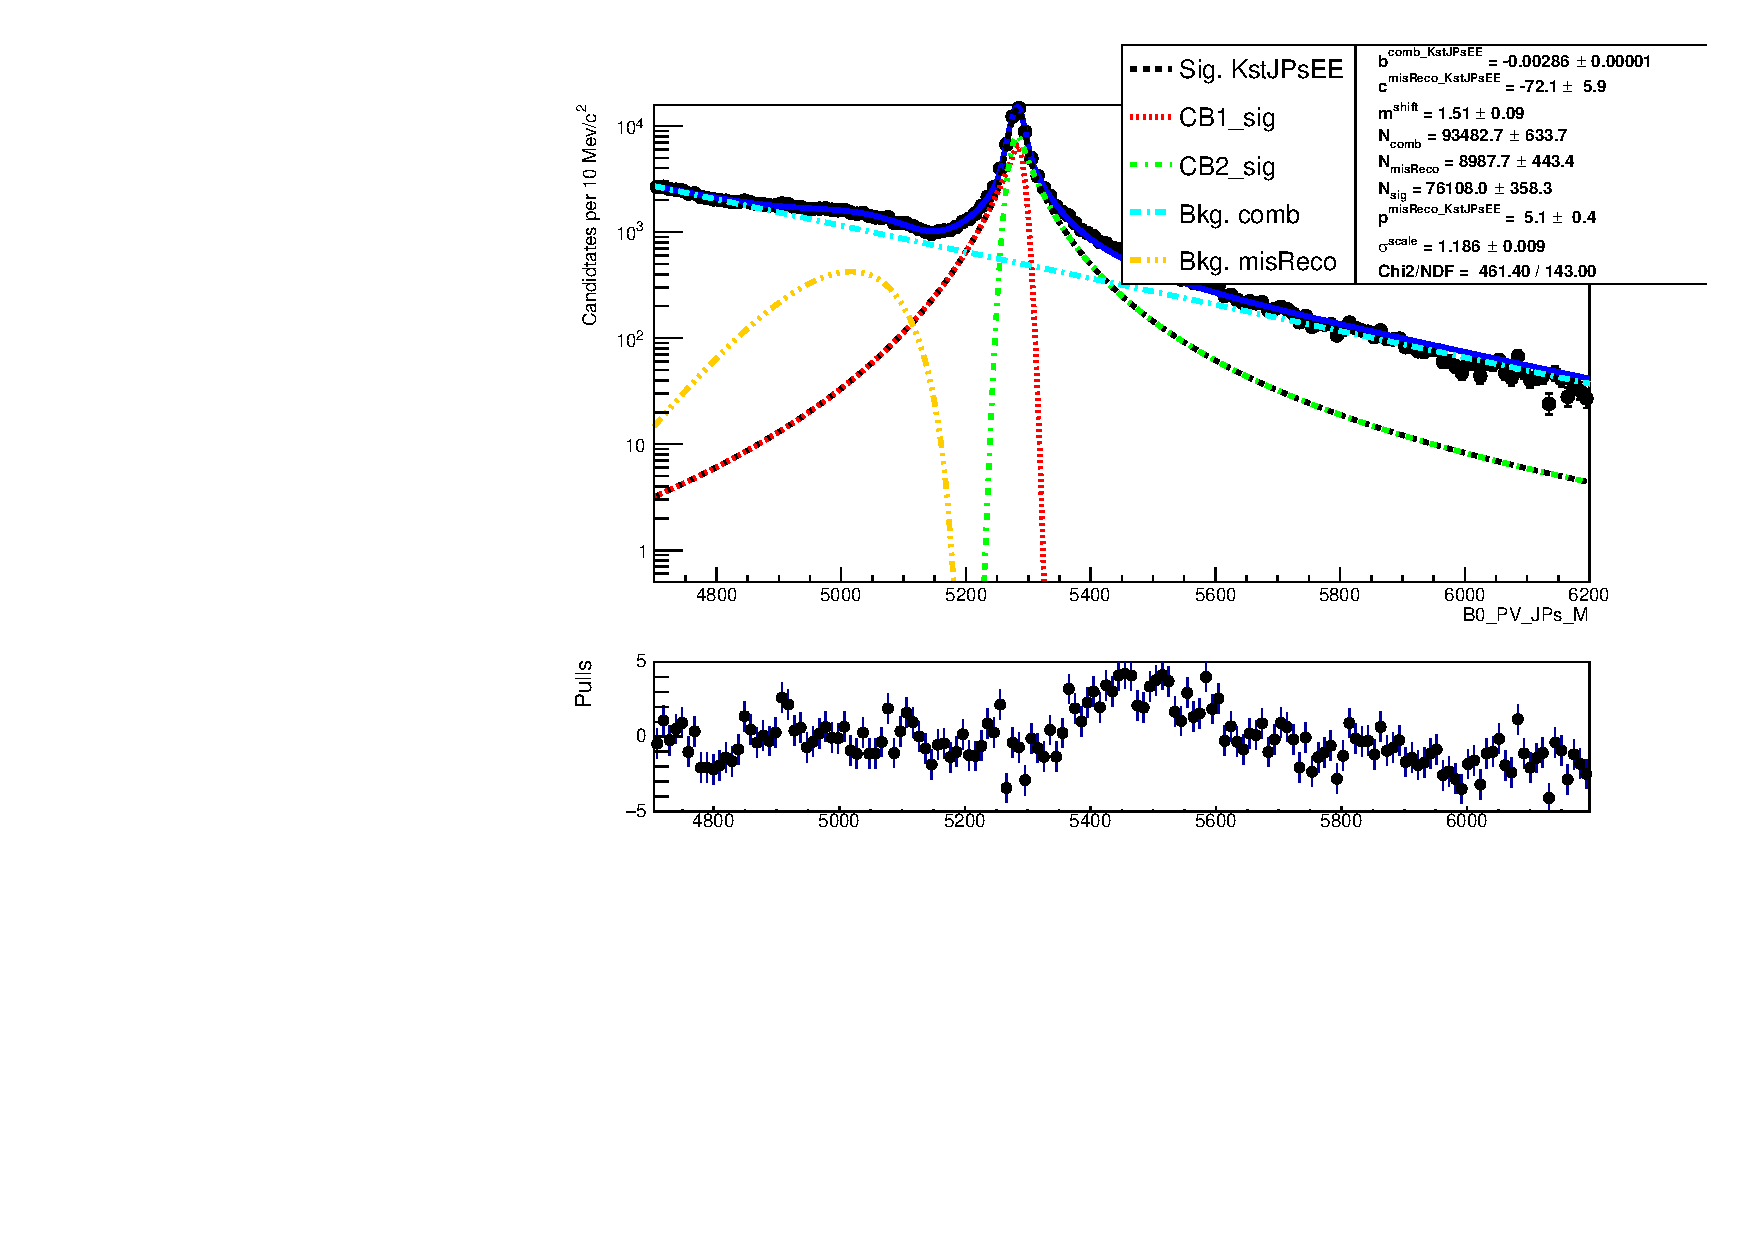
\includegraphics[width=0.48\textwidth]{RKst/figs/sW/KstJPsEE_log_fitAndRes.pdf}
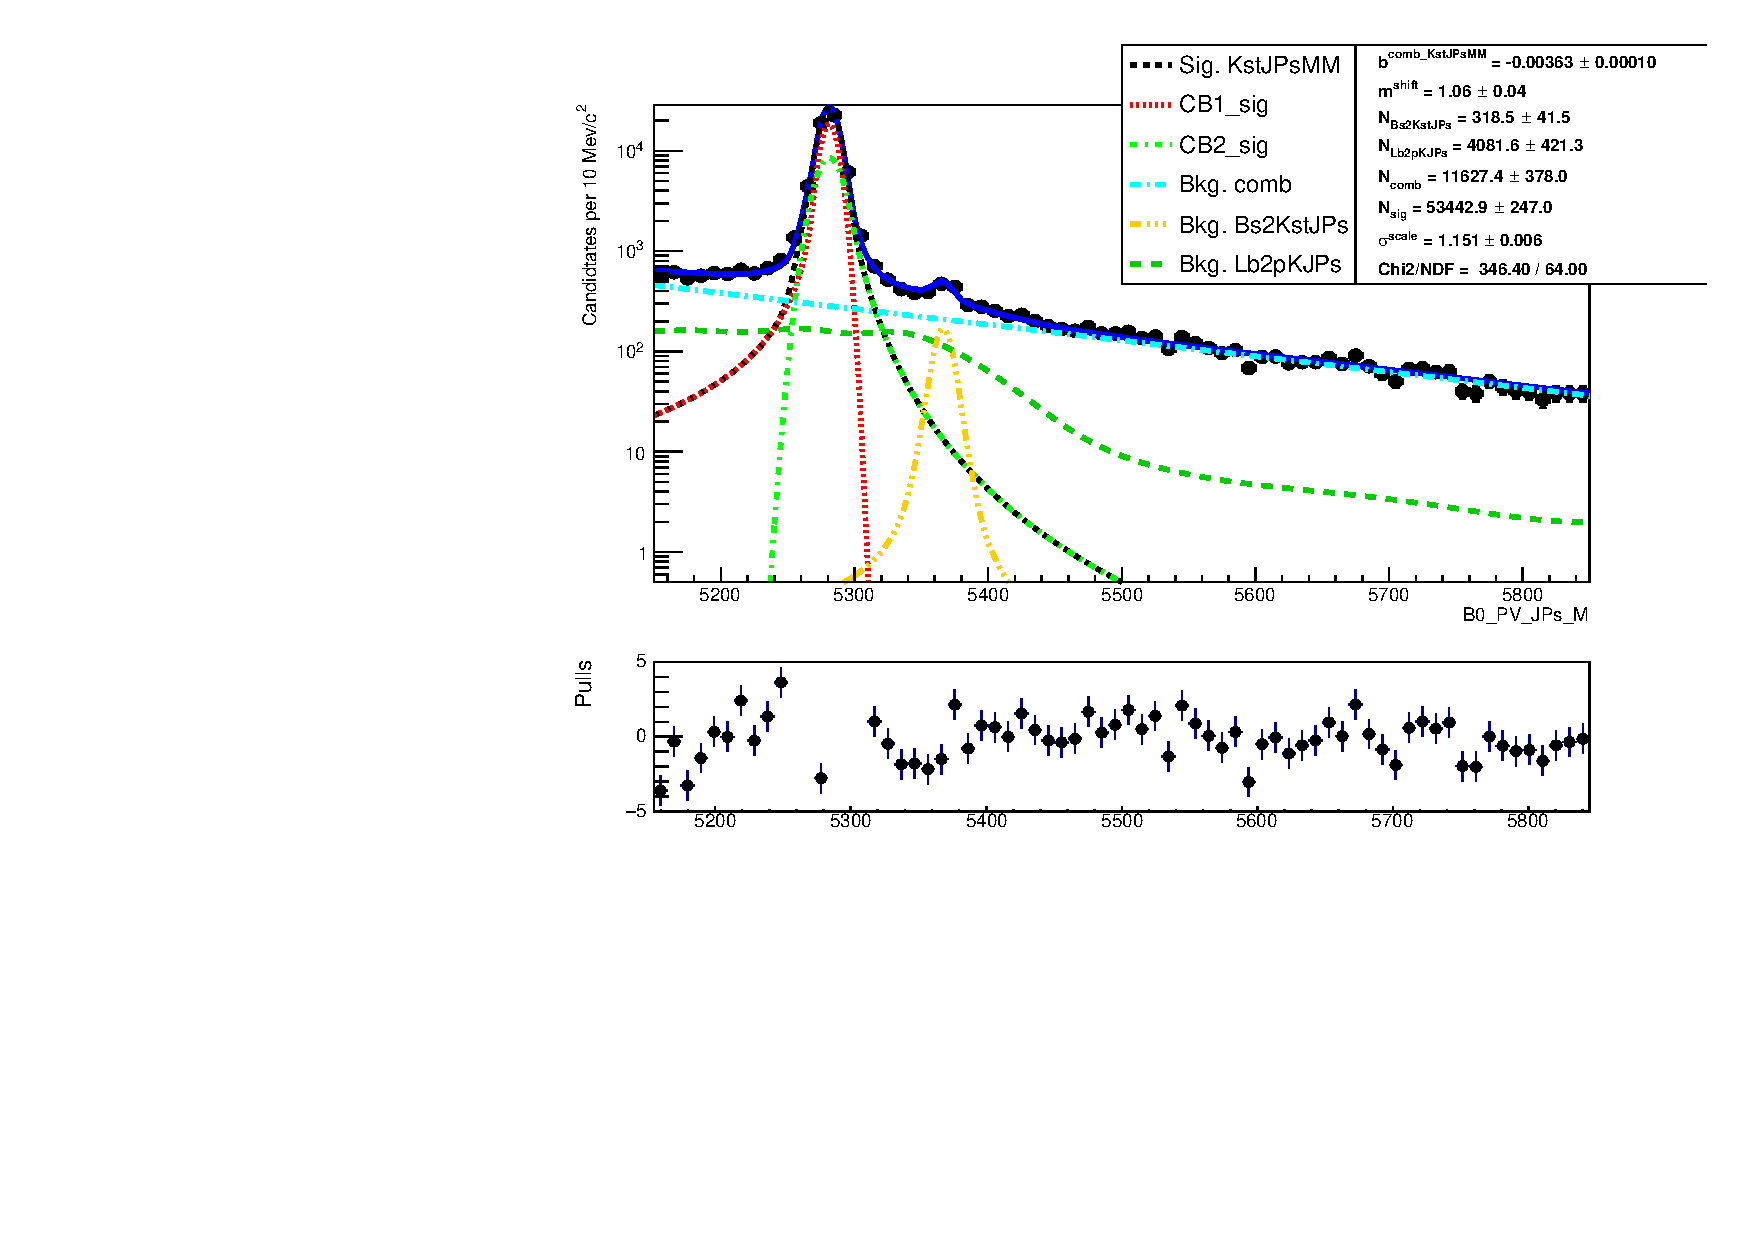
\includegraphics[width=0.48\textwidth]{RKst/figs/sW/KstJPsMM_log_fitAndRes.pdf}
\caption{Fitted 4-body invariant mass distributions after pre-selection 
for the electron (left) and muon (right) channels.}
\label{fig:RKst_sW_mass}
\end{figure}

 \begin{figure}[h!]
\centering
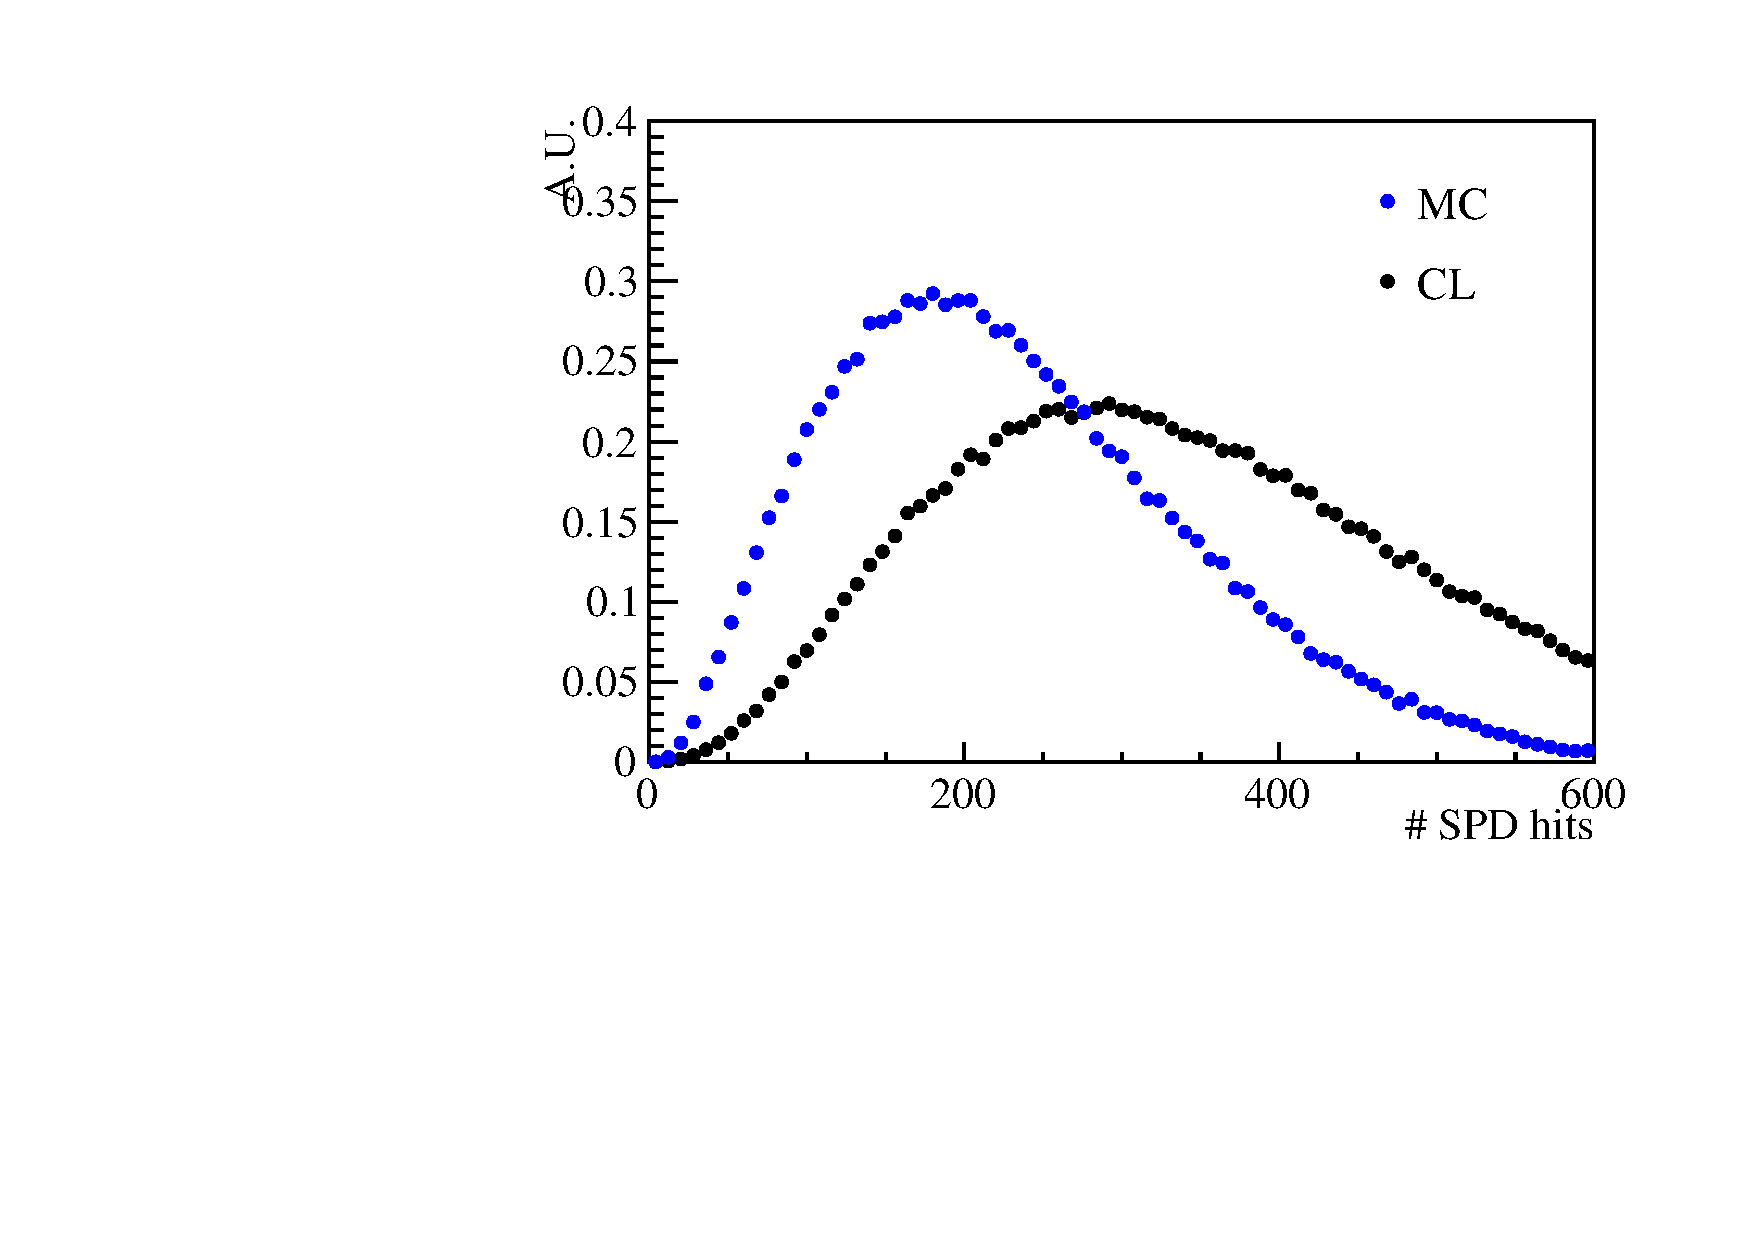
\includegraphics[width=0.48\textwidth]{RKst/figs/nspd_12.pdf}
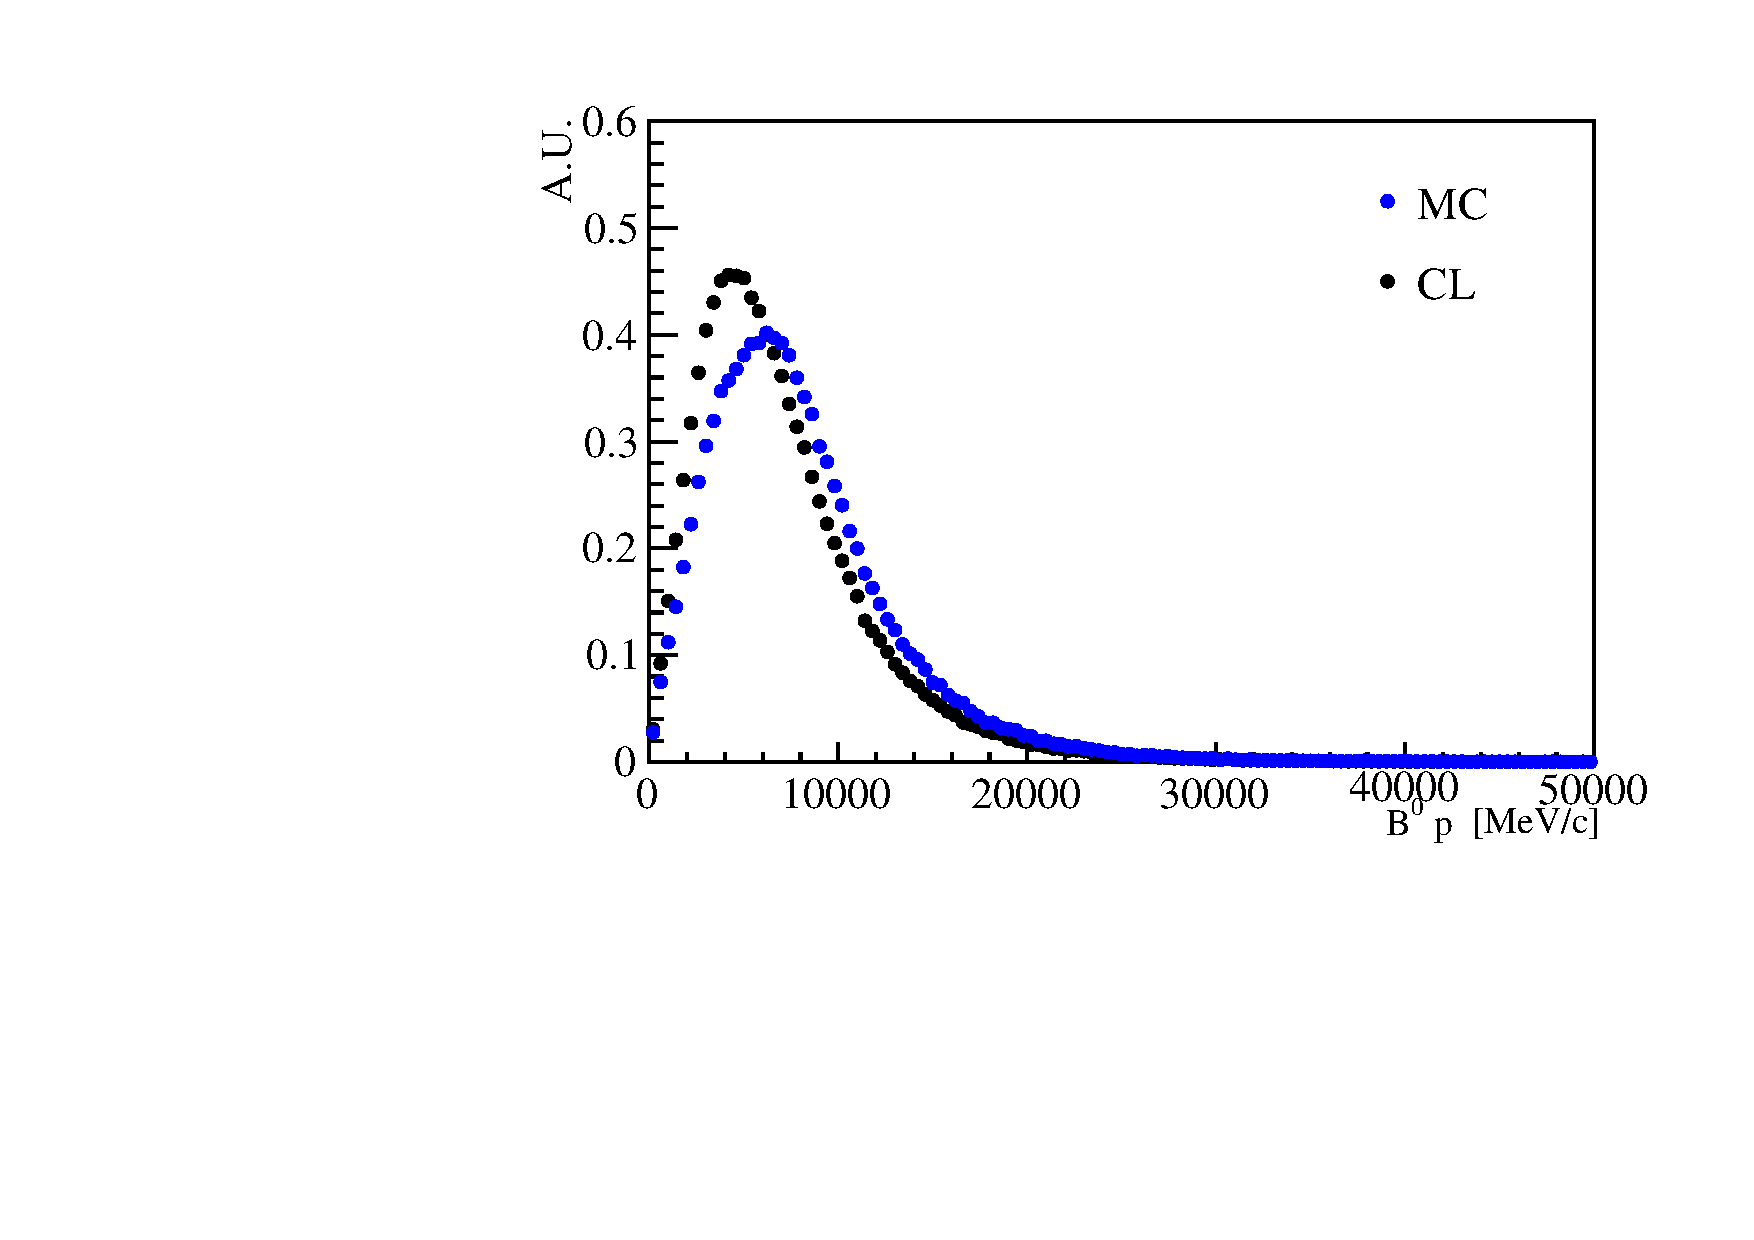
\includegraphics[width=0.48\textwidth]{RKst/figs/bpt.pdf}
\caption{Distributions of number of SPD hits (left) and \Bz transverse momentum (right) in data and MC.}
\label{fig:b0pt_nSPD_distrib}
\end{figure}

\begin{figure}[h!]
\centering
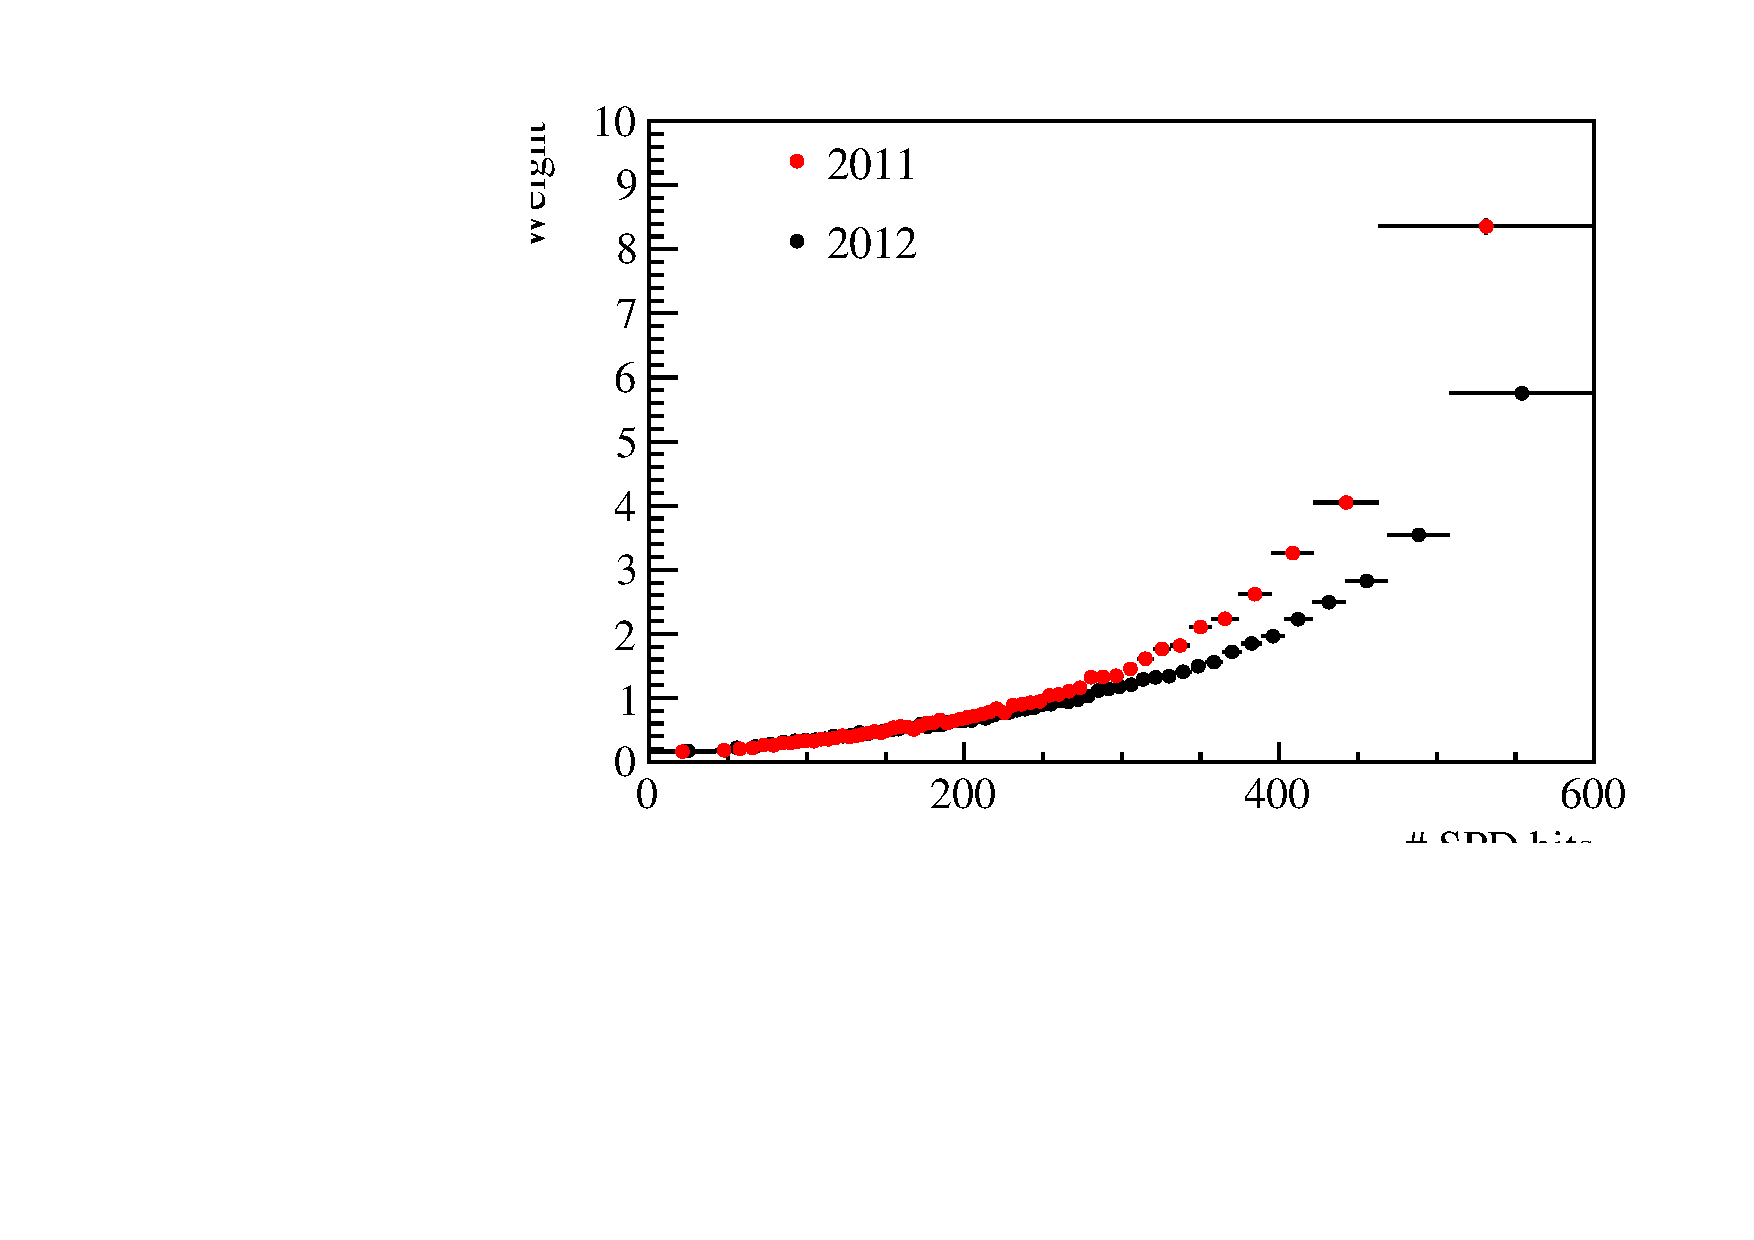
\includegraphics[width=0.48\textwidth]{RKst/figs/nspd_w.pdf}
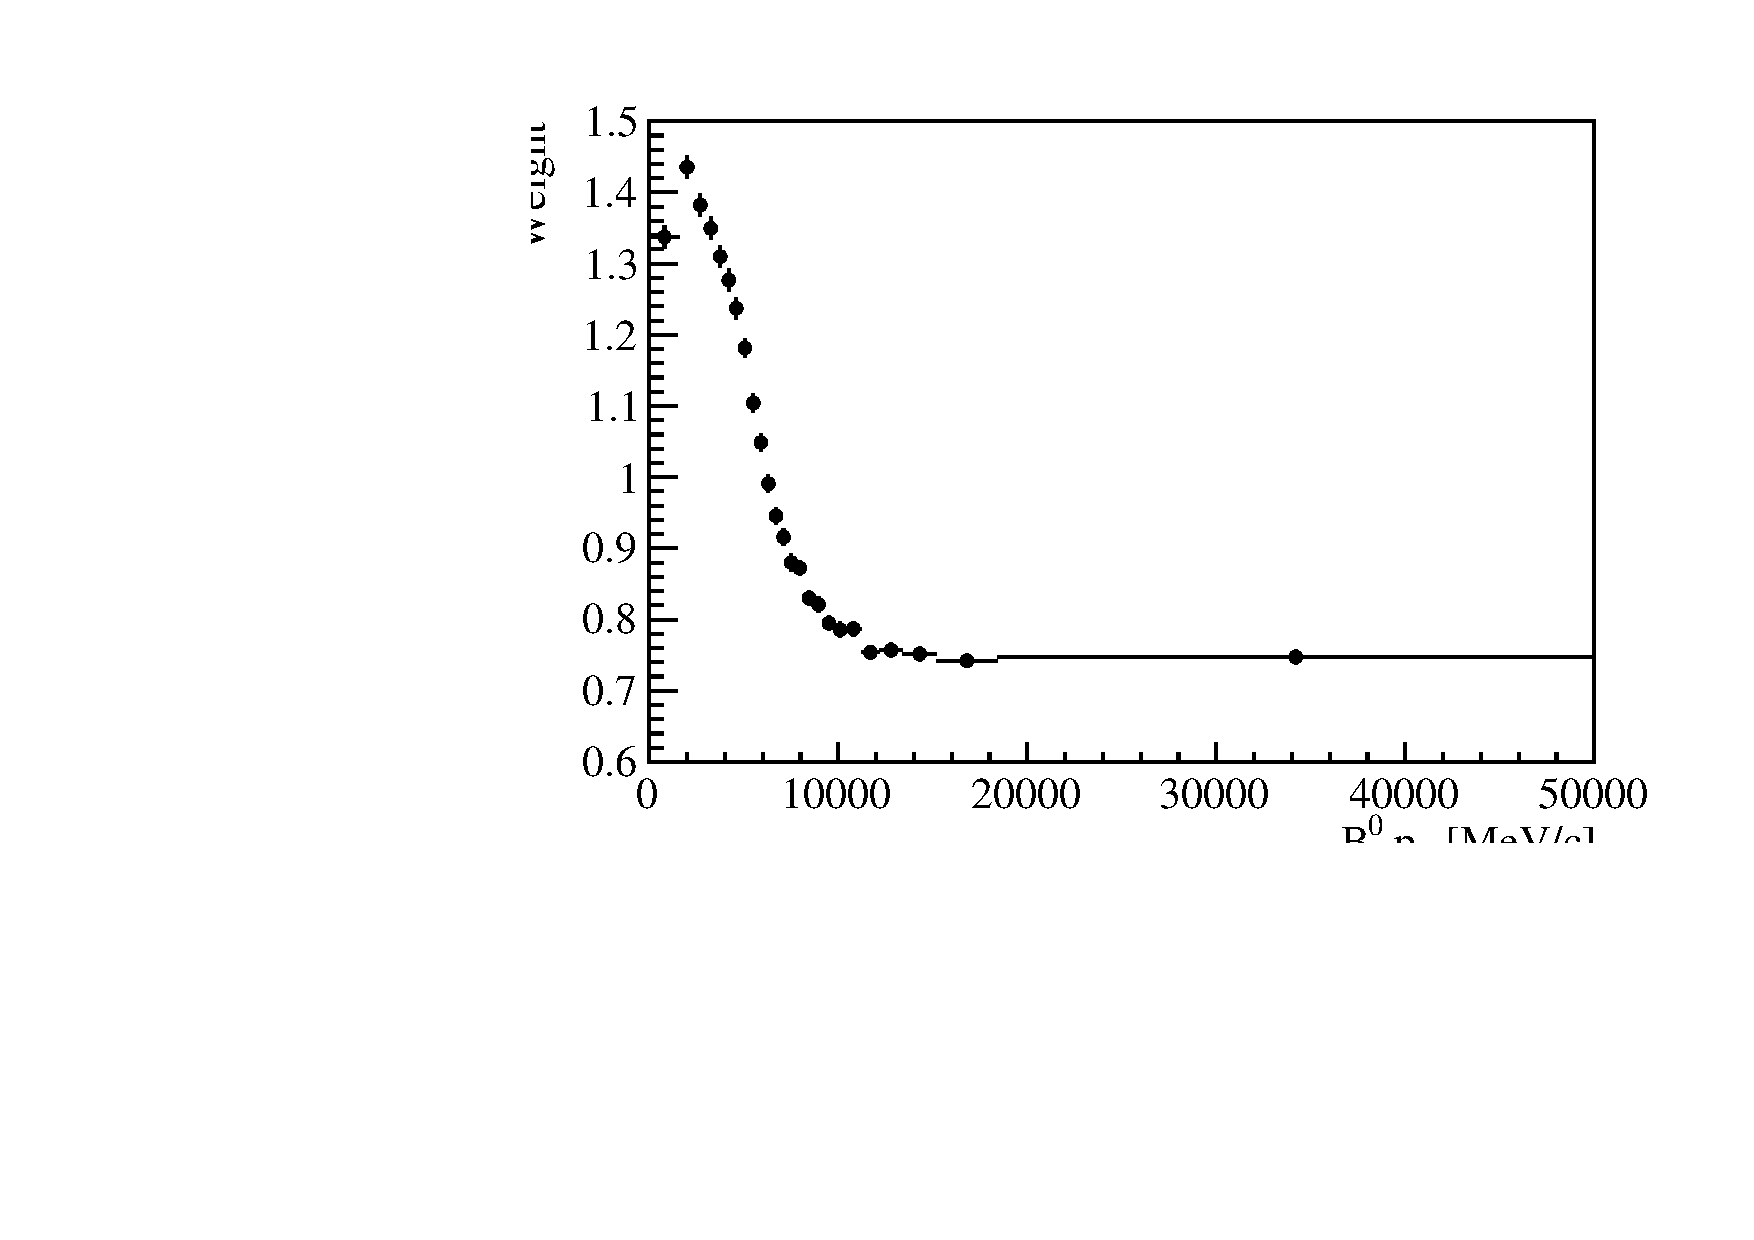
\includegraphics[width=0.48\textwidth]{RKst/figs/bpt_w.pdf}
\caption{ Ratios of simulated over real data distributions used to correct the Monte Carlo
as a function of the number of SPD hits (left) and the \Bz transverse momentum (right). }
\label{fig:b0pt_nSPD_ratios}
\end{figure}

%\begin{figure}[h!]
%\centering
%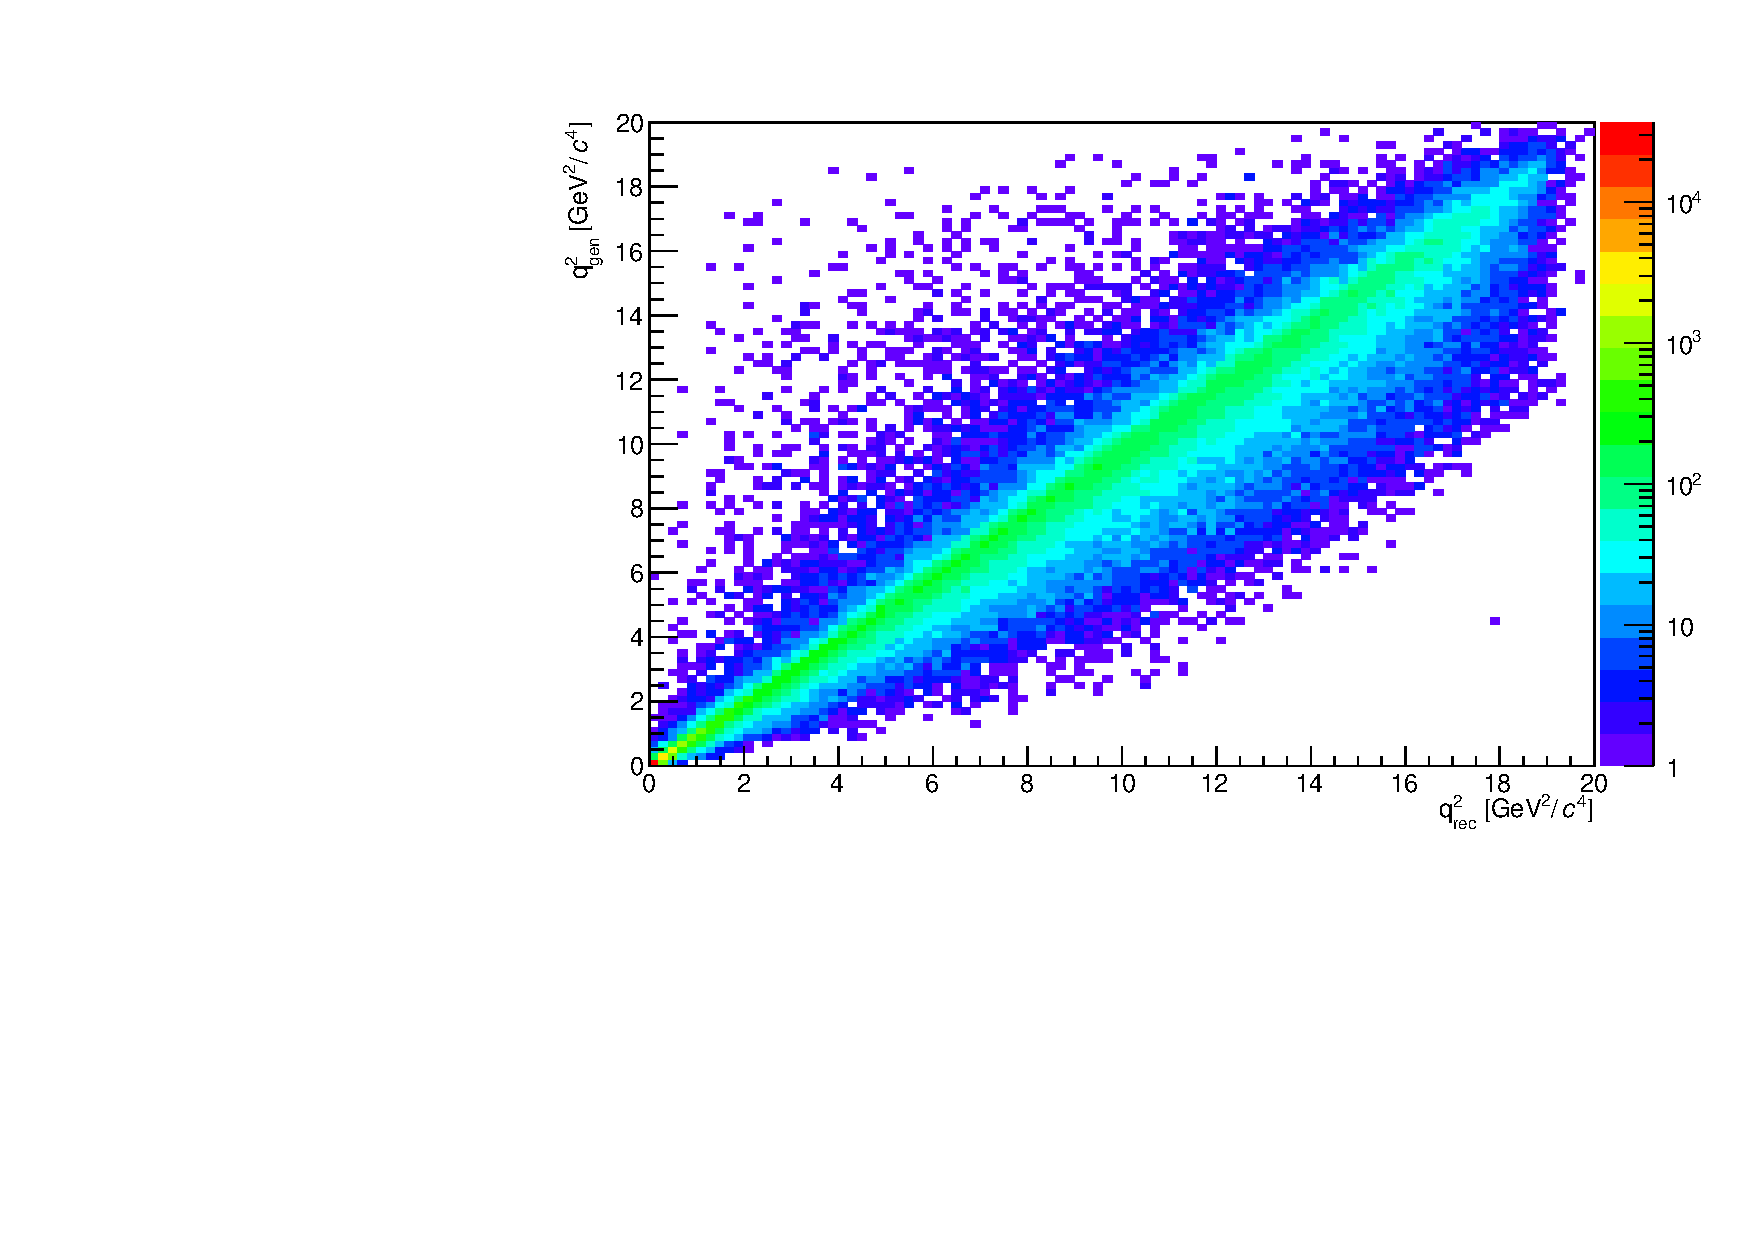
\includegraphics[width=0.48\textwidth]{RKst/figs/bin_mig.pdf}
%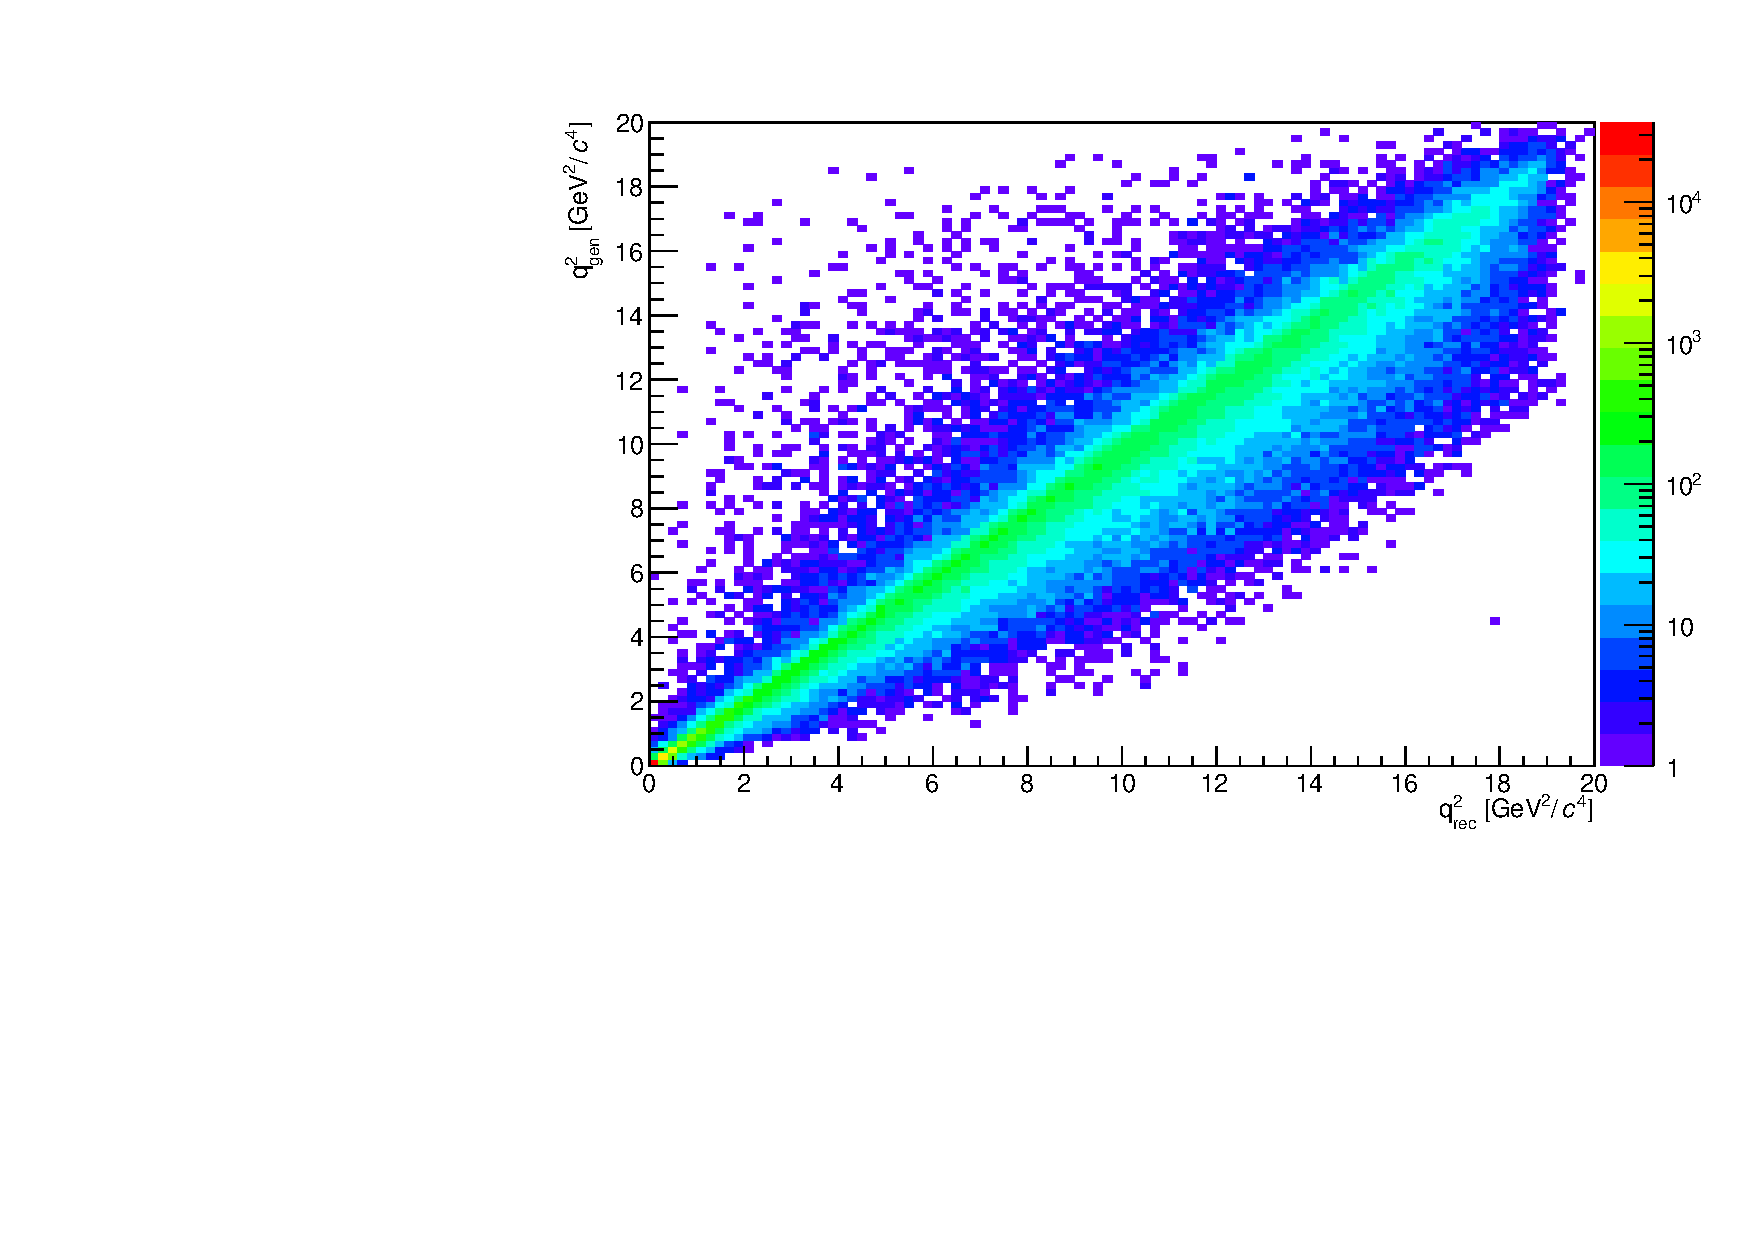
\includegraphics[width=0.48\textwidth]{RKst/figs/bin_mig.pdf}
%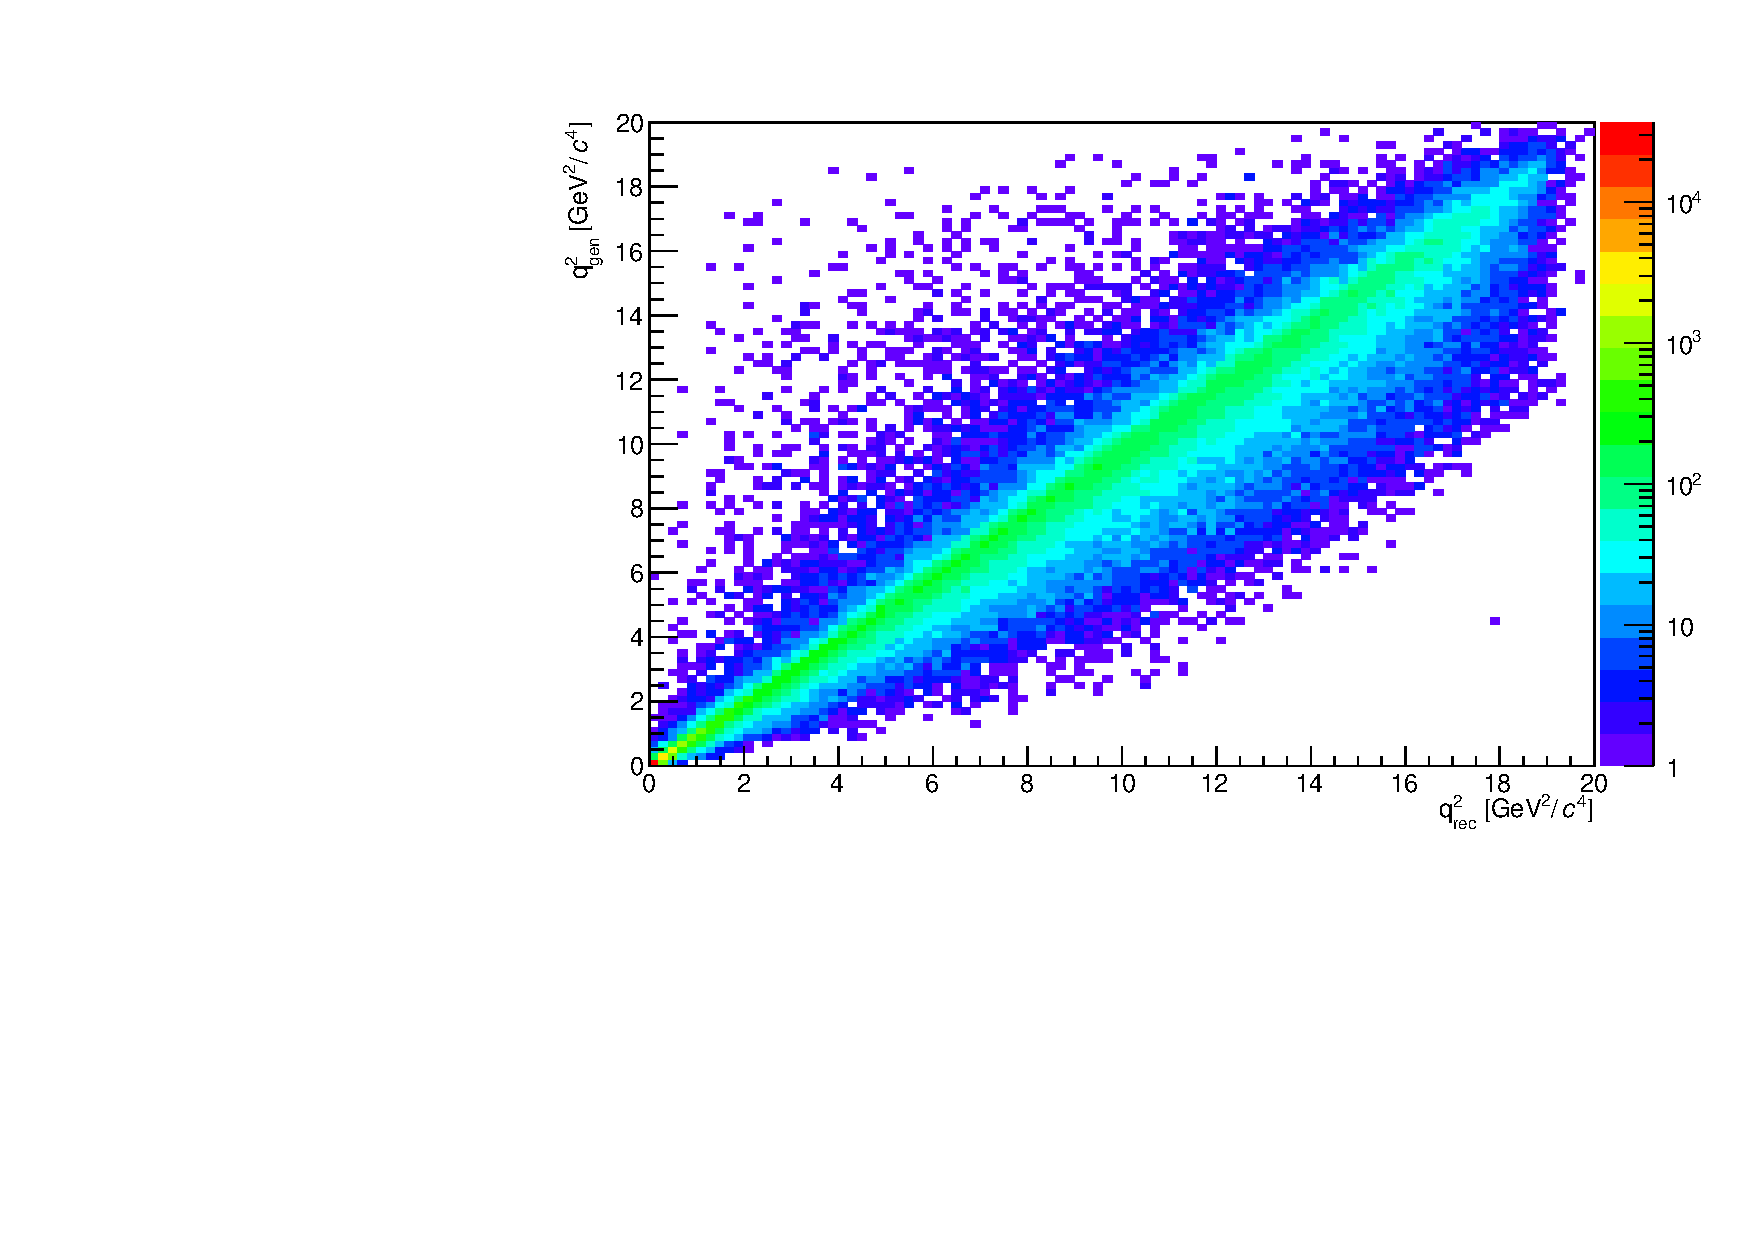
\includegraphics[width=0.48\textwidth]{RKst/figs/bin_mig.pdf}
%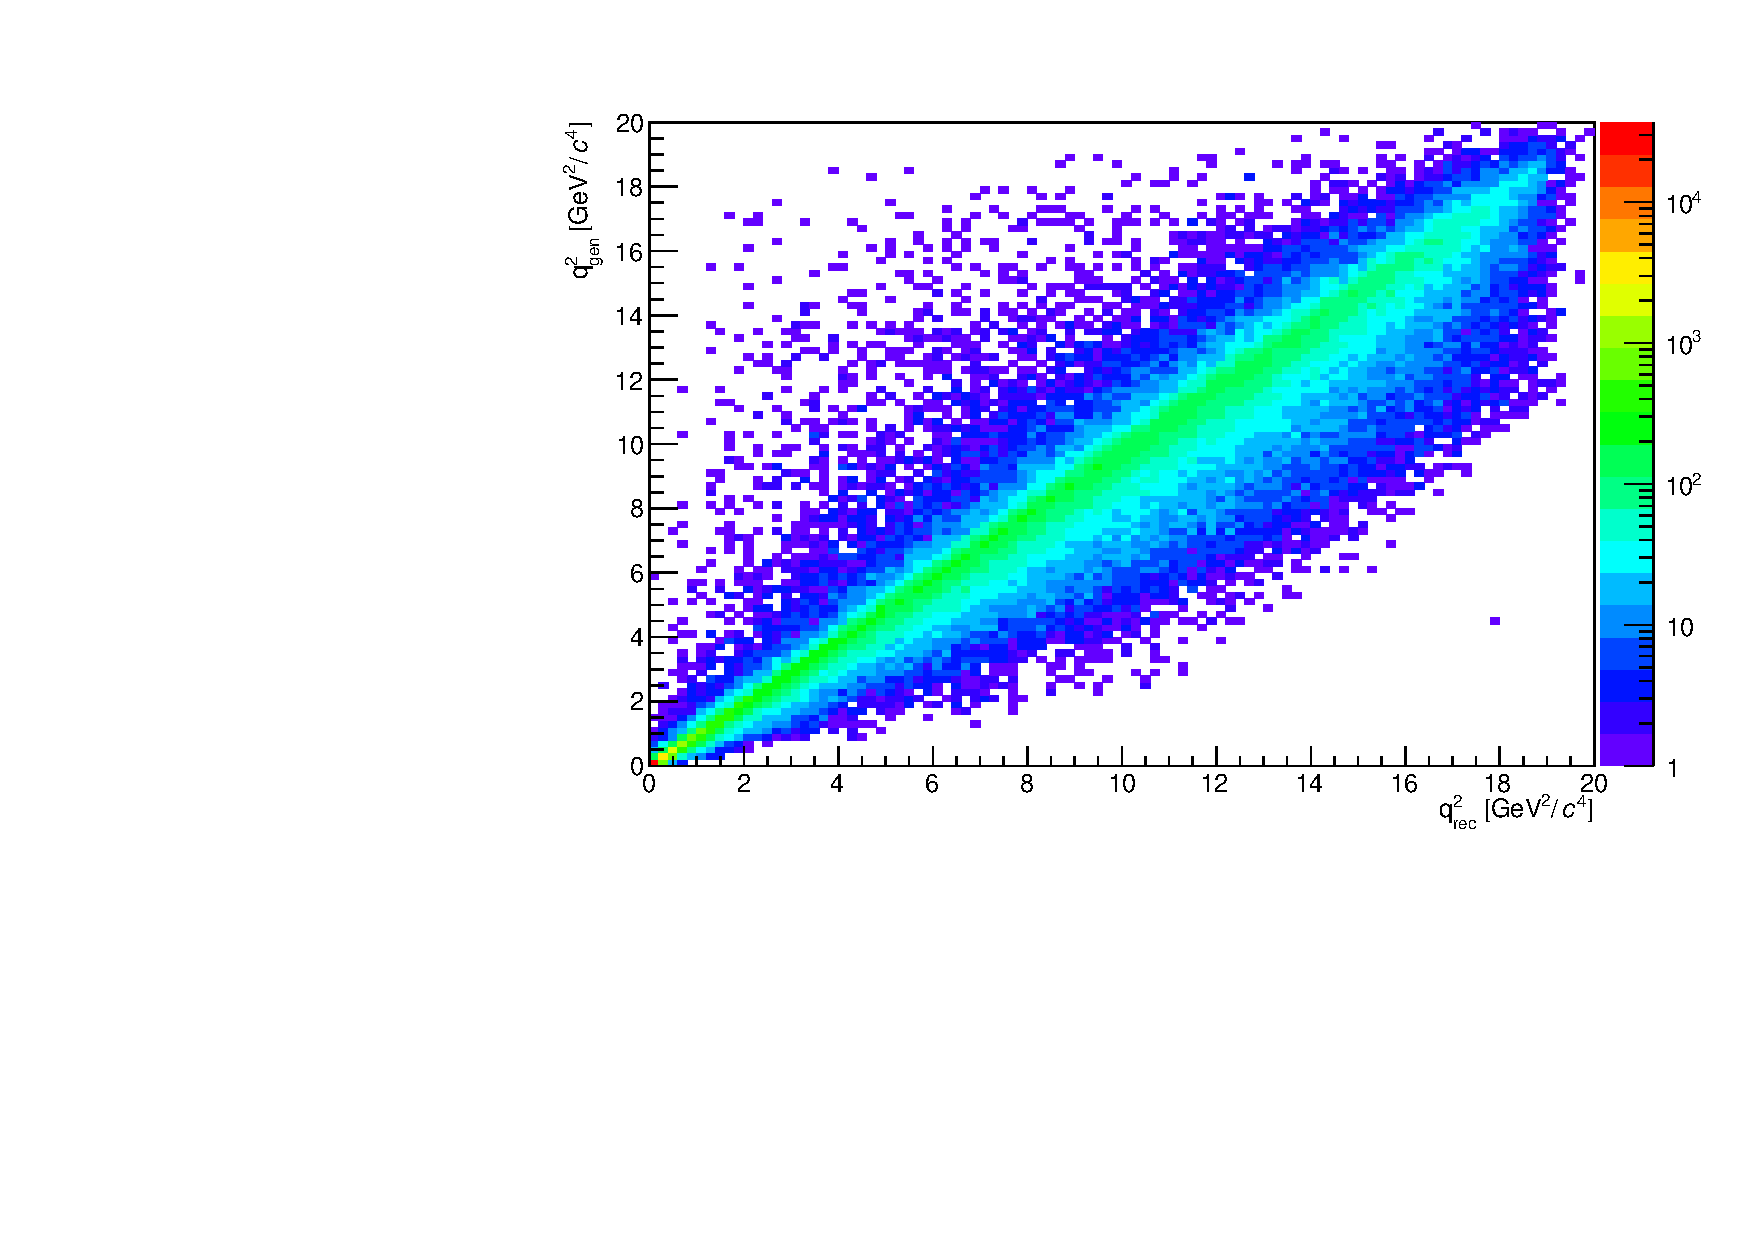
\includegraphics[width=0.48\textwidth]{RKst/figs/bin_mig.pdf}
%\caption{Generated versus reconstructed \qsq in simulated $\decay{\Bz}{\Kstar ee}$ events.}
%\label{fig:ee_bin_mig}
%\end{figure}


\section{Geometric efficiency}


The simulated samples used contain the requirement that daughters are in the LHCb
detector acceptance. This corresponds to the requirement for each of the final particles
to have polar angle $\theta$ between 10 and 400 mrad. The efficiency of this
cuts is obtained using a generator level Monte Carlo sample.

\section{Reconstruction efficiency and bin migration}

The reconstruction efficiency is here defined as the efficiency to reconstruct
each decay channel given that its daughters are into the geometrical acceptance
of the detector. This includes both the probability that a particle generates
observable signatures and the efficiency of all the preselection cuts described in Sec.~\ref{sec:RKst_selection},
including those done to remove peaking backgrounds. This efficiency is evaluated on simulated events
to which the full list of weights described in Sec.~\ref{sec:RKst_weights} is applied.
The efficiency of the PID cuts is kept separate as it is known to be not well simulated
and there are reliable data-driven methods which can be used to extract it (see Sec.~\ref{sec:RKst_pid_eff}).

One effect which must be considered is the ``bin migration", namely the possibility
that events generated in a \qsq interval will be reconstructed in a different one.
Two different effects can cause bin migration. First of all an imperfect resolution
can cause events at the edges of the considered interval to fall on the wrong side of the edge.
This effect is only important in case of non-flat true distributions, as the amount of bin migration
in the two directions is different.
The second possible source of bin migration are systematic effects due, for example,
to the presence of bremsstrahlung photons that cannot be reconstructed.
It is particularly important to take the bin migration into account in the electron channels case 
because the \qsq resolution is worse and at the same time more photons are radiated from the final state.
Figure~\ref{fig:ee_bin_mig} shows the correlation between reconstructed and generated \qsq
in simulated $\decay{\Bz}{\Kstar ee}$ events. In the ideal case of perfect resolution this plot
would look like a diagonal line and in the case of no bias its slope would be 1.
Table \ref{tab:bin_mig} reports net bin migration amounts in the considered \qsq intervals.
The reconstruction efficiency is calculated comparing generated to reconstructed samples
and therefore already includes bin migration effects. Nevertheless, it is useful to single
out this component in order to be able to asses systematic uncertainties.

\begin{figure}[h!]
\centering
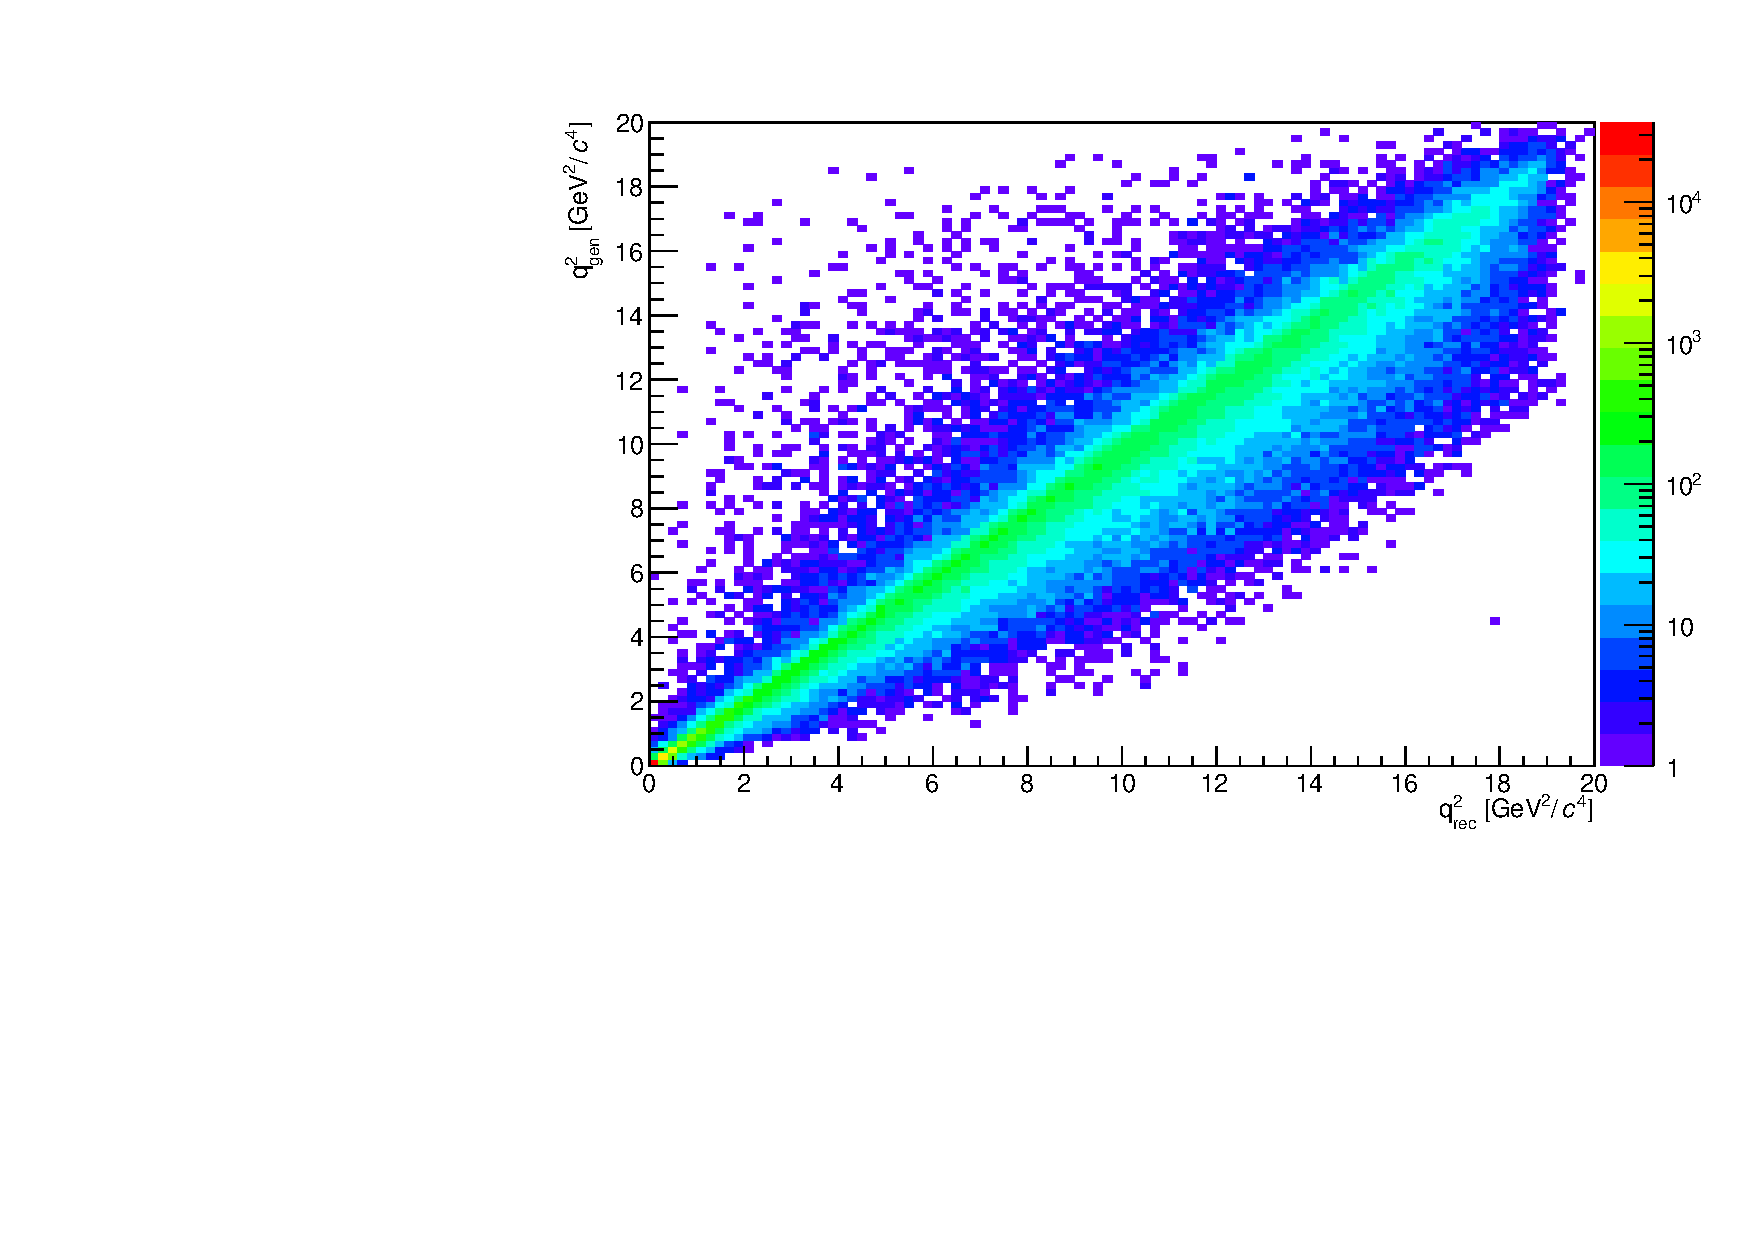
\includegraphics[width=0.85\textwidth]{RKst/figs/bin_mig.pdf}
\caption{Generated versus reconstructed \qsq in simulated $\decay{\Bz}{\Kstar ee}$ events.}
\label{fig:ee_bin_mig}
\end{figure}

\begin{table}[bh]
\label{tab:bin_mig}
\centering
\begin{tabular}{|c|c|c|c|}
\hline
 Sample 			& 1--6 GeV$^2/c^4$ 				& 15--20 GeV$^2/c^4$ 				& $J/\psi$  \\ \hline
$\mu\mu$ 	& $ -0.0018  \pm  0.0002 $ & $ 0.0042  \pm  0.0003 $ & $ -0.0012  \pm  0.0000 $ \\
$ee$ 	& $ 0.0834  \pm  0.0013 $ & $ -0.4469  \pm  0.0091 $ & $ -0.0258  \pm  0.0003 $ \\
\hline 
 \end{tabular}
\caption{Net bin migration amounts in the considered \qsq intervals.
Positive values mean ``net in", negative values ``net out".}
\end{table}

\section{PID efficiency}
\label{sec:RKst_pid_eff}

The Monte Carlo is known not to reliably describe particle ID variables
and therefore a data-driven method is used to obtain this efficiency component.
Furthermore the same method is used to weight the MC in order to extract MVA and trigger efficiencies.

In order to do this the PIDCalib package~\cite{Aaij:1978280} was used. This tool uses decays where final 
particles can be identified thanks to their kinematic properties.
For example $\KS\to\pi^+\pi^-$ has a clear signature with a displaced vertex
and can be easily singled out from other decays and used to test pion PID efficiency.
The narrow peaks of the $\jpsi\to\mumu$ and $\jpsi\to\ee$ decays allow to calibrate
muon and electron efficiencies. Finally, $\phi\to KK$ and $\D^*\to D(\to K\pi)\pi$ decays
are used to test the kaon efficiency. Residual background in this decays is subtracted using
the $_s\mathcal{P}$lot technique~\cite{sPlot}.

The package allows to divide the phase-space in bins and obtain a data-driven efficiency for each bin.
For this analysis the phace-space was divided in equi-popolated bins of momentum
and pseudorapidity of the particle under study. Figure~\ref{fig:pid_perf_hist} shows performance
tables for pions, kaons, muons and electrons.

The decay channel under study genrally has different kinematical distributions than the calibration sample.
Therefore, once the efficiency table is obtained for each particle, the total efficiency for each candidate
is calculated as the product of the four final particles efficiencies.
$\varepsilon^{ev} = \varepsilon_K\cdot\varepsilon_\pi\cdot\varepsilon_{\ell_1}\cdot\varepsilon_{\ell_2}$.
Finally, the total efficiency is found by averaging over all simulated events.

\begin{equation}
\varepsilon_{PID} = \frac{1}{N} \sum_i^N \varepsilon_K(p_K^i,\eta_K^i) \cdot \varepsilon_\pi(p_\pi^i,\eta_\pi^i) \cdot \varepsilon_\ell(p_{\ell_1}^i,\eta_{\ell_1}^i) \cdot \varepsilon_K(p_{\ell_2}^i,\eta_{\ell_2}^i)
\end{equation}

\begin{figure}[h!]
\centering
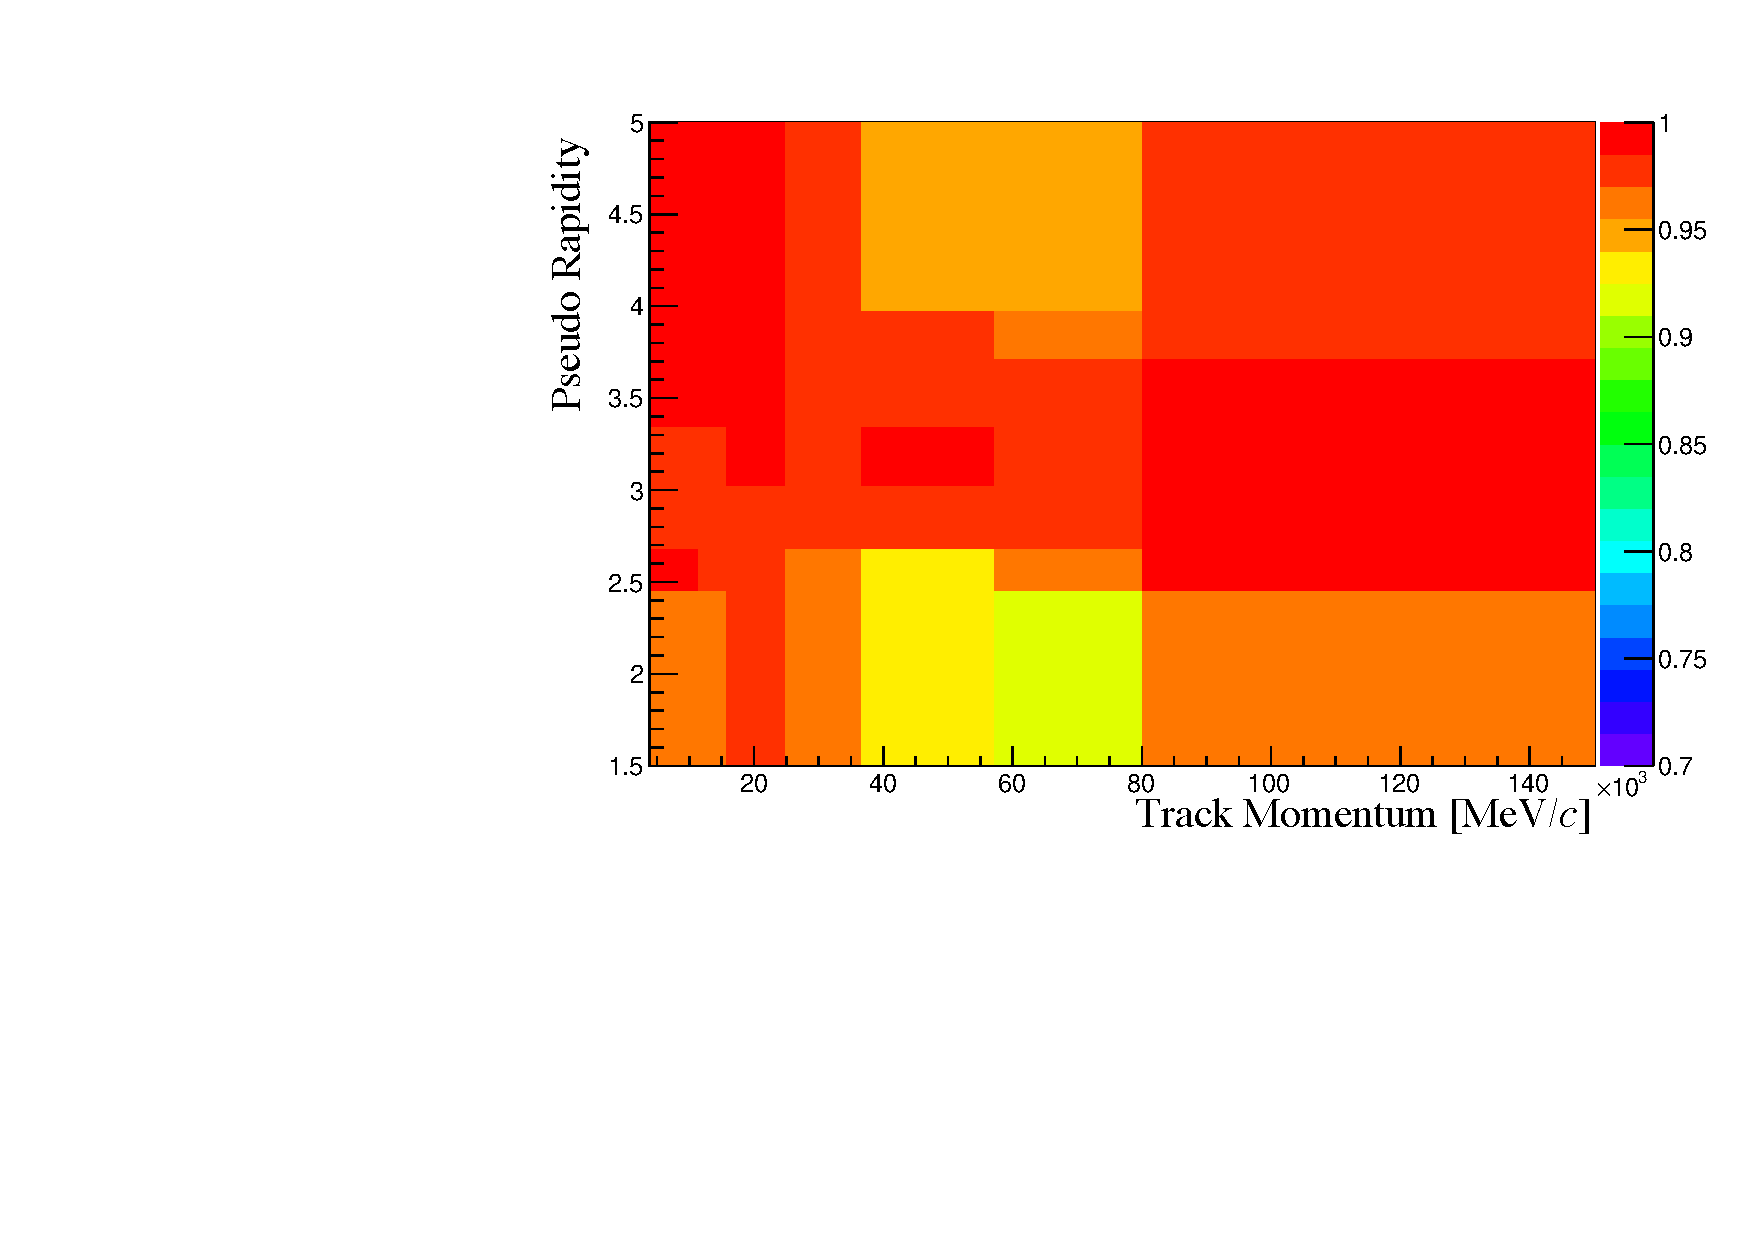
\includegraphics[width=0.48\textwidth]{RKst/figs/pid_Pi.pdf}
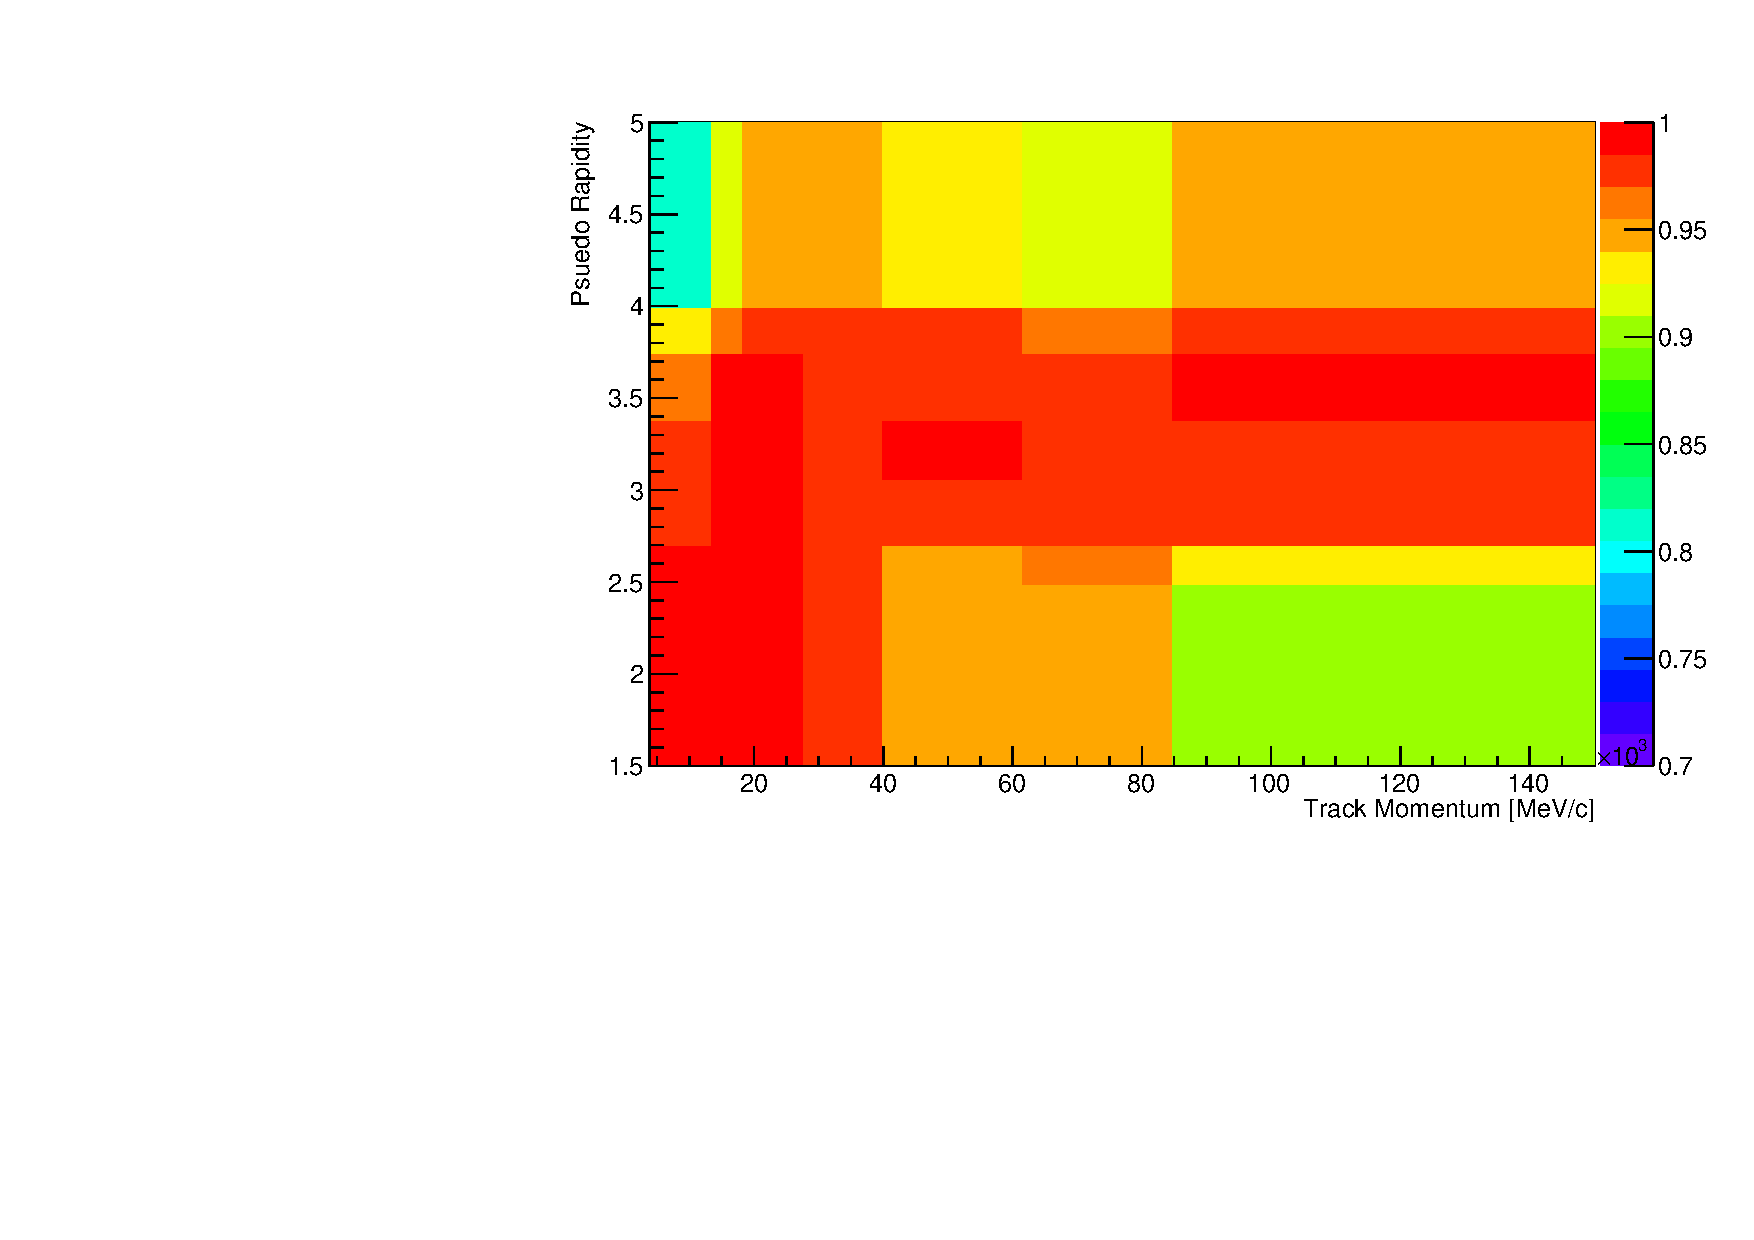
\includegraphics[width=0.48\textwidth]{RKst/figs/pid_K.pdf}
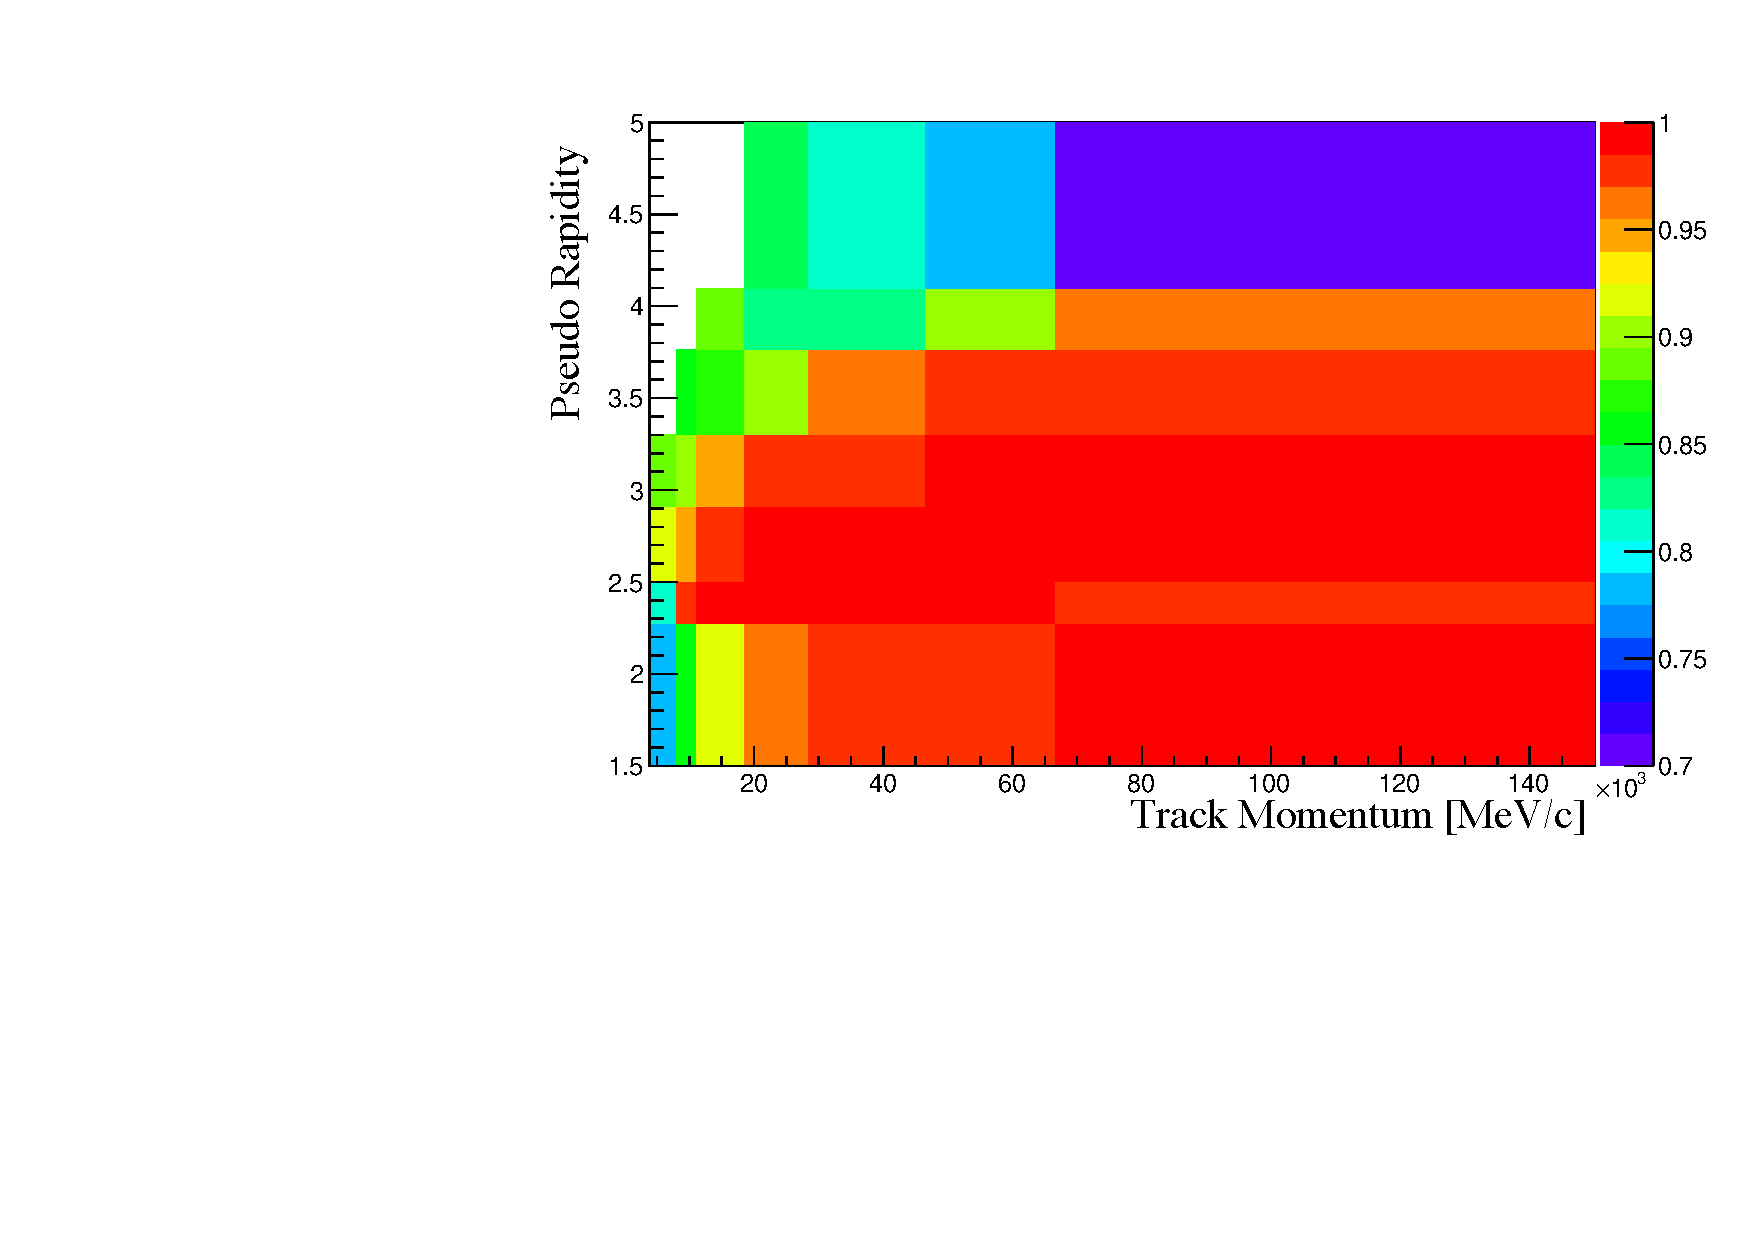
\includegraphics[width=0.48\textwidth]{RKst/figs/pid_Mu.pdf}
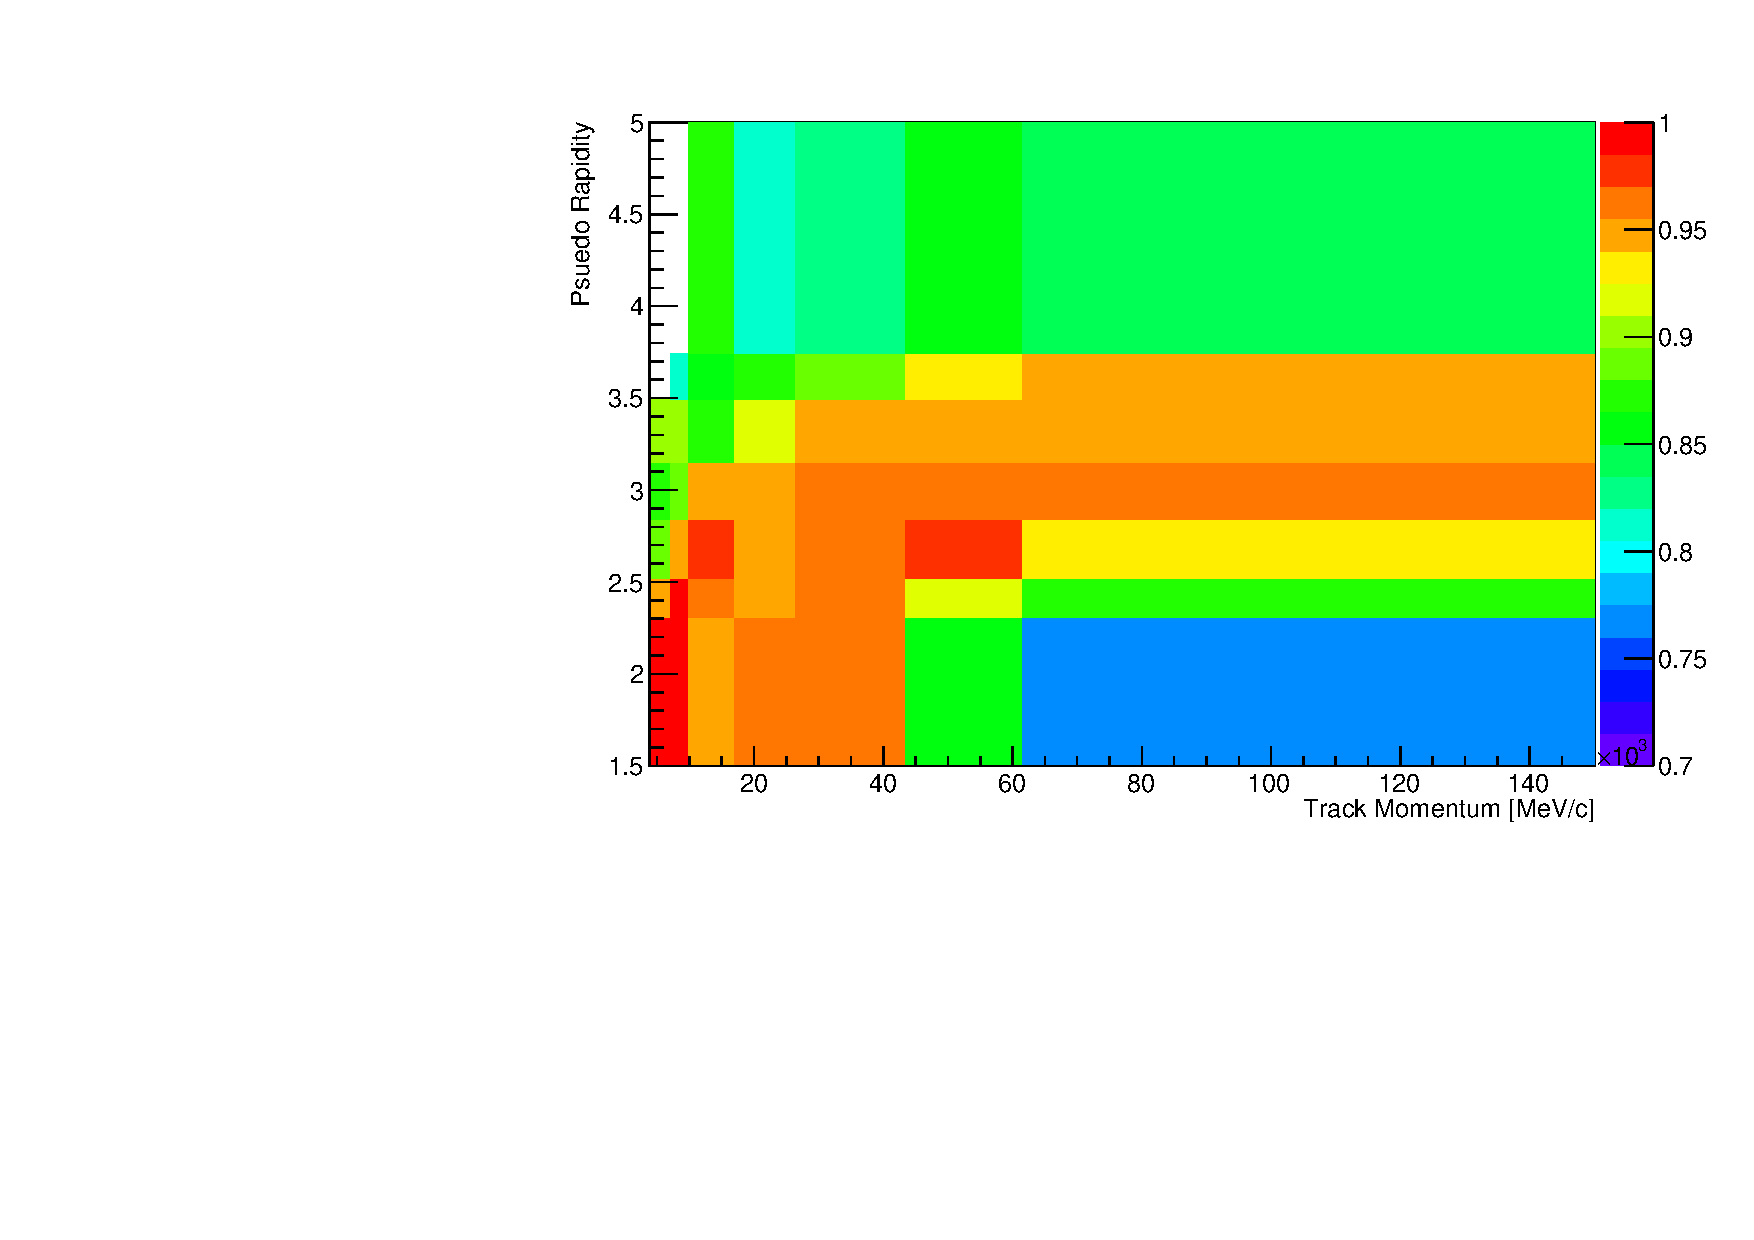
\includegraphics[width=0.48\textwidth]{RKst/figs/pid_e.pdf}
\caption{Performance tables obtained with data-driven methods
for pions (top left), kaons (top right), muons (bottom left) and electrons (bottom right).}
\label{fig:pid_perf_hist}
\end{figure}


\section{Trigger efficiency}
\label{sec:RKst_trigger_eff}

\subsection{Muonic channels}

For the muonic channels the trigger efficiency is calculated using simulated events.
Using the resonant channel the efficiency obtained using the simulation
was crosschecked with the data driven TISTOS method as already described in Sec.~\ref{sec:Lb_trigger_eff}.

%In LHCb triggered events can fall in two categories: events triggered by a track which is part
%of the decay of interest, Trigger On Signal (TOS), or by other tracks in the events,
%Trigger Independent of Signal (TIS). All trigger lines used for this analysis are required to be TOS.
%The efficiency for TOS trigger can be obtained by data by the following formula:
%\begin{equation}
%\varepsilon_{TOS} = \frac{TOS \mbox{ and } TIS}{TIS}
%\end{equation}

{\em Results of TISTOS}

%For 2011 we use the official 0x40760037 TCK, corresponding to 0.944 \invfb of data.
%For 2012 the official TCK is 0x409f0045 describes only data after the June technical stop (1.442 \invfb).
%Samples with different TCKs are weighted to respect the percentage of luminosity taken with each configuration.

\subsection{Electronic channels}

For the electronic channels data is fitted separately in three trigger categories: L0Electron, L0Hadon and L0TIS.
Therefore we need to extact the efficiency separately for each category.

While the Hlt (1 and 2) efficiency is still computed using simulated events,
the L0Electron and L0Hadron efficiencies cannot be modelled with the Monte Carlo.
The discrepancy between data and simulation is mainly due to the ageing of the 
calorimeters, on which the decision of these triggers relies. The ageing is not simulated
in the Monte Carlo and affects the L0 trigger efficiency which, therefore, must
be calibrated using data driven-methods. Tables of efficiencies are obtained
applying the TIS-TOS method to a calibration sample.

For each trigger category these tables contain efficiency as a function of
\pt of the considered particle and are given for different calorimeter regions
as these have different properties (e.g. cell size) due to the different position
with respect to the beam line. Regions considered are inner and outer HCAL, and inner, middle and outer ECAL.
Figure~\ref{sec:L0eff_tables} shows data-driven efficiencies for the L0Electron trigger
in the three ECAL regions.

\begin{figure}[h!]
\centering
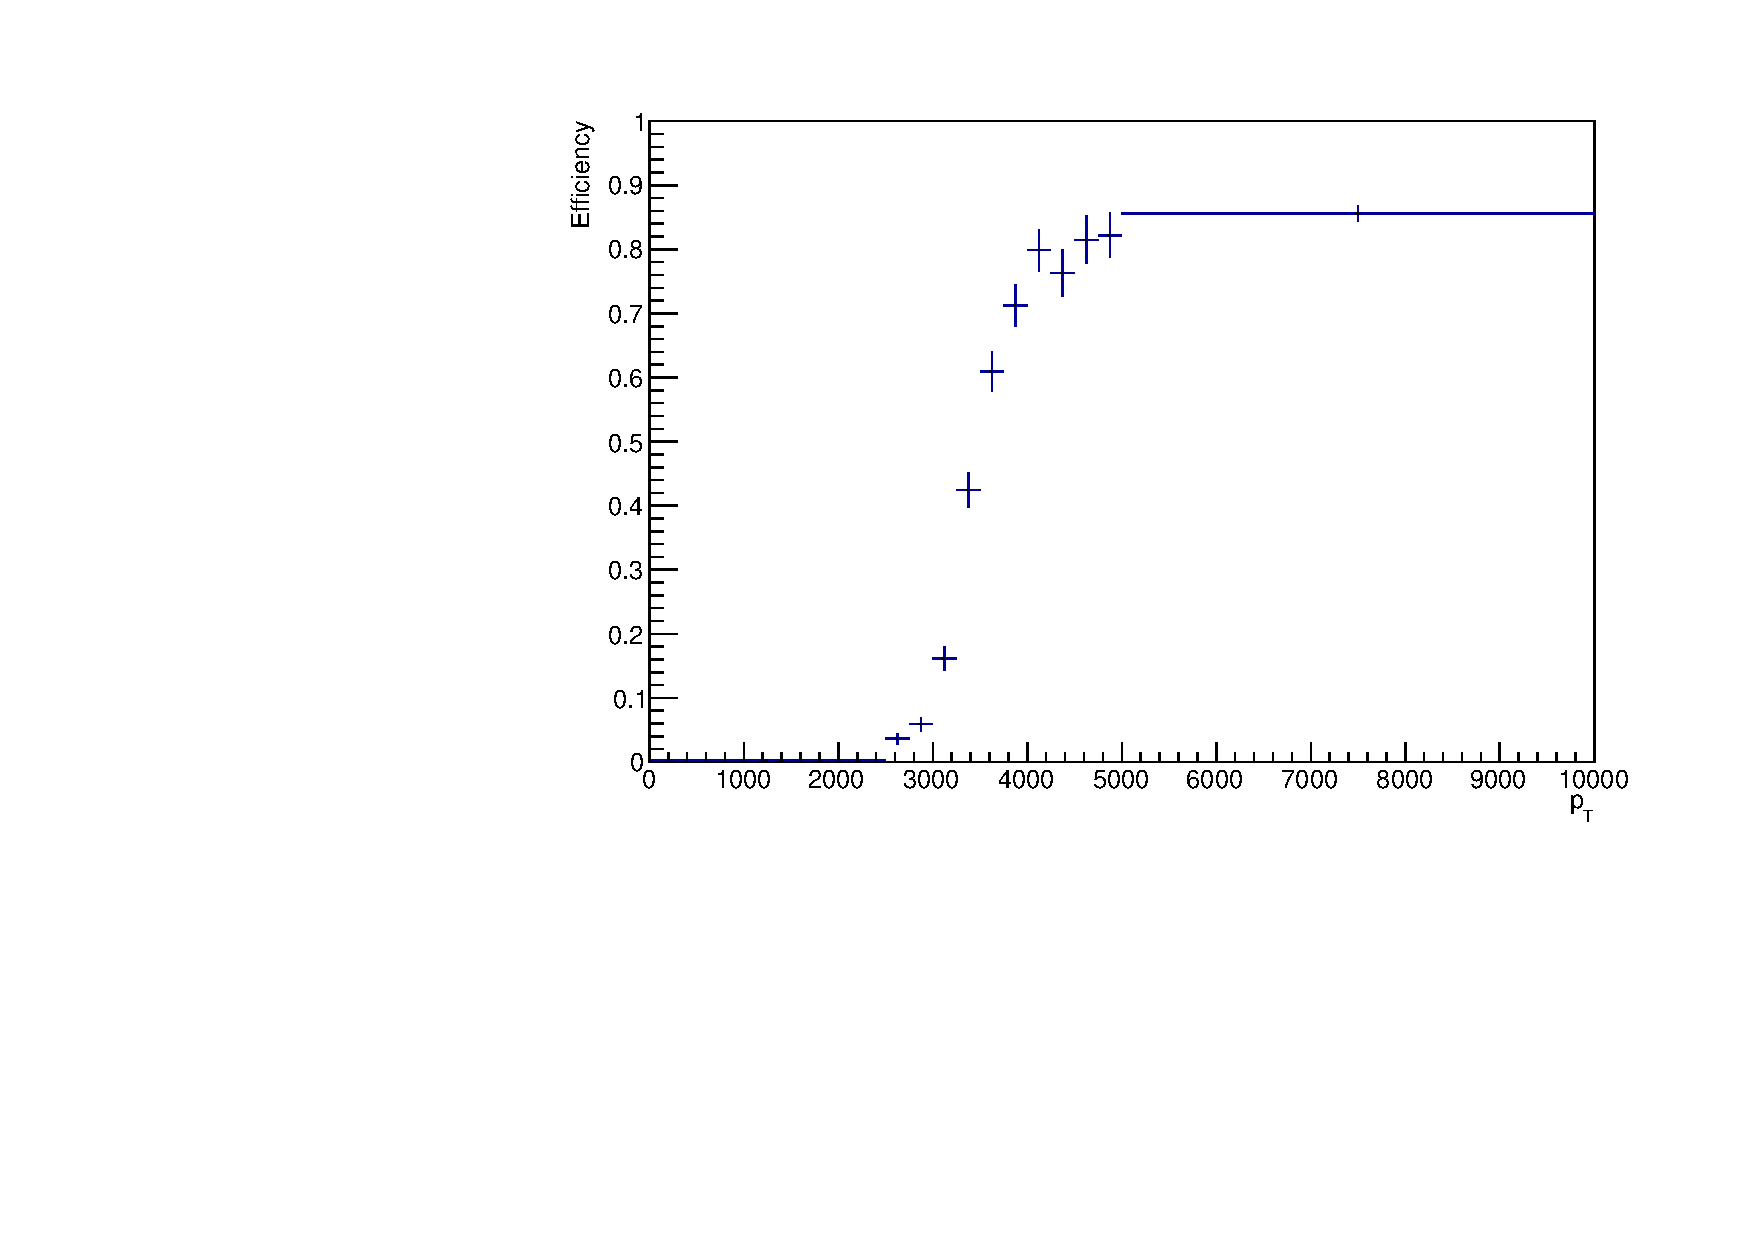
\includegraphics[width=0.48\textwidth]{RKst/figs/l0plots/l0E_Inner.pdf}
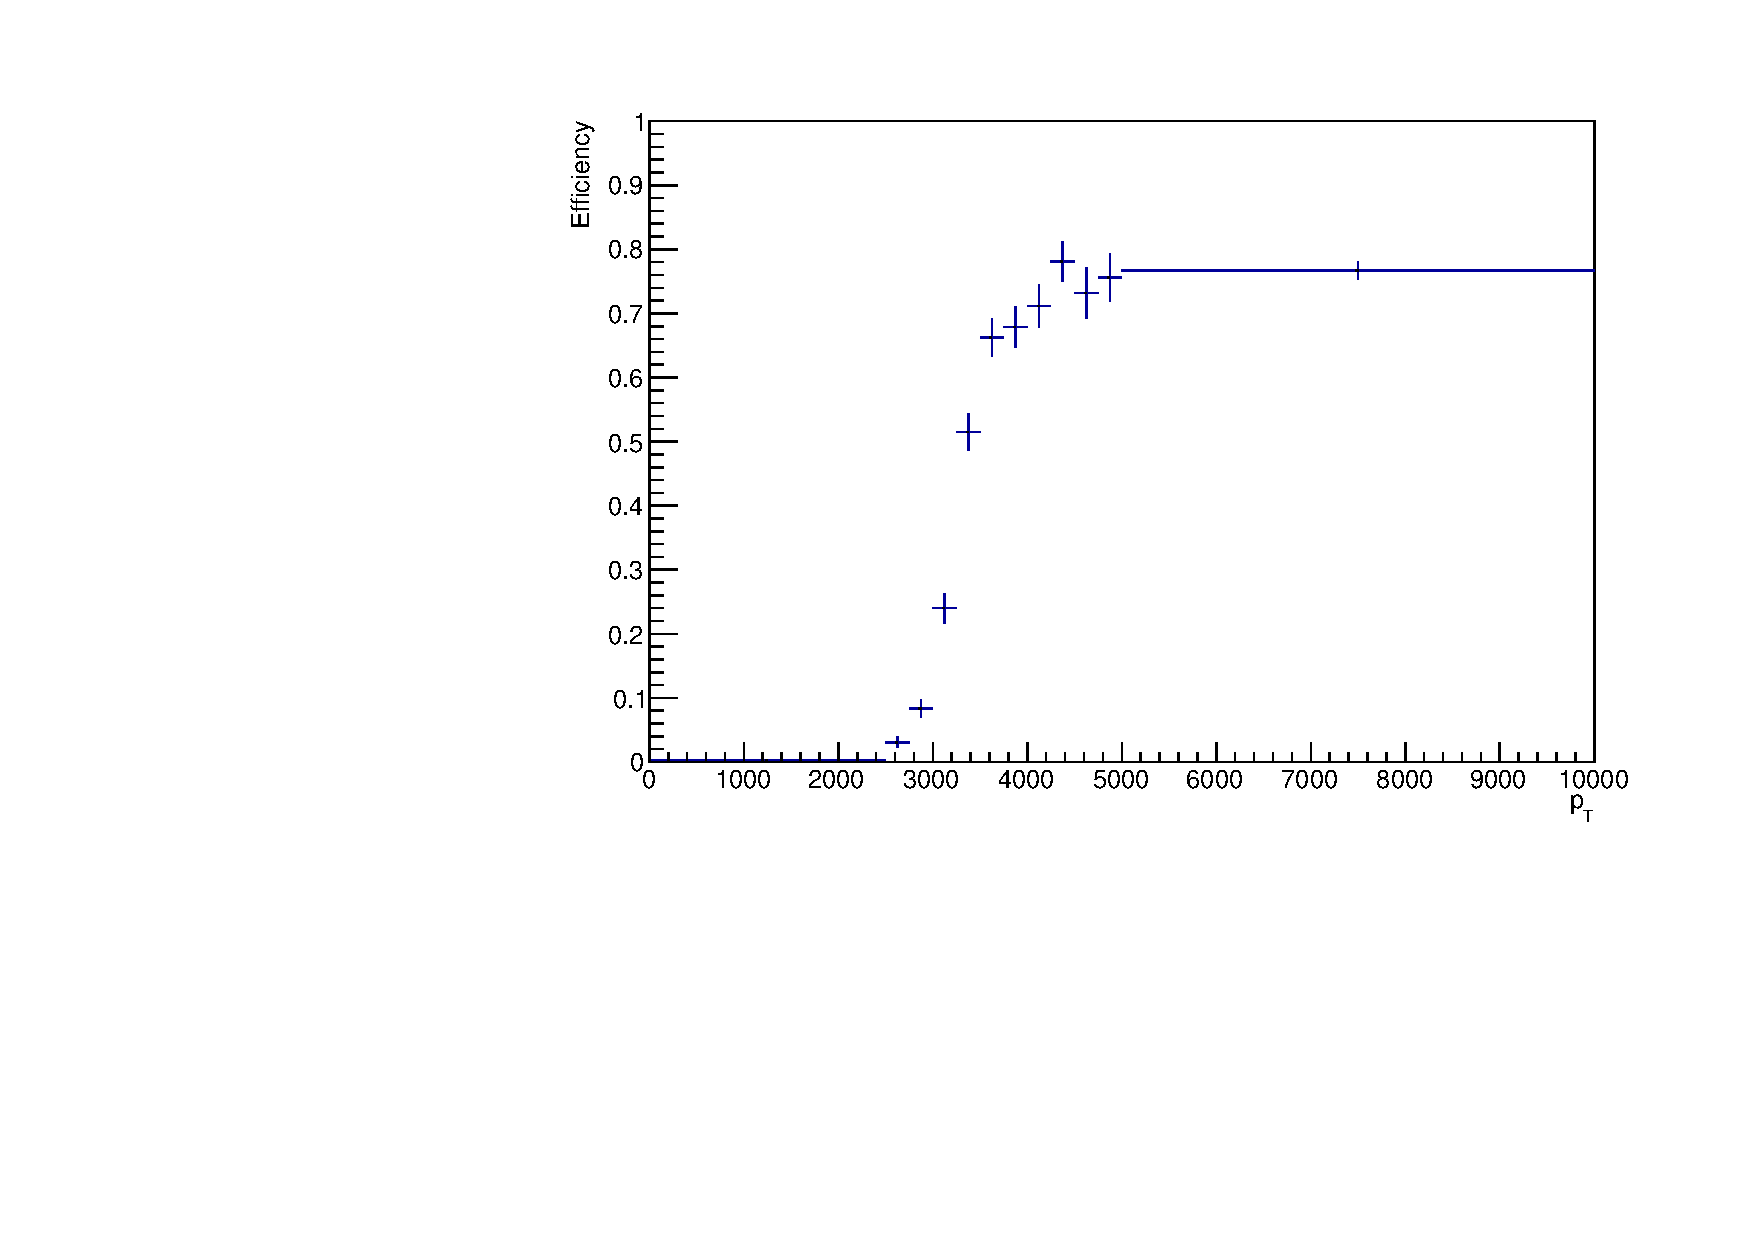
\includegraphics[width=0.48\textwidth]{RKst/figs/l0plots/l0E_Middle.pdf}
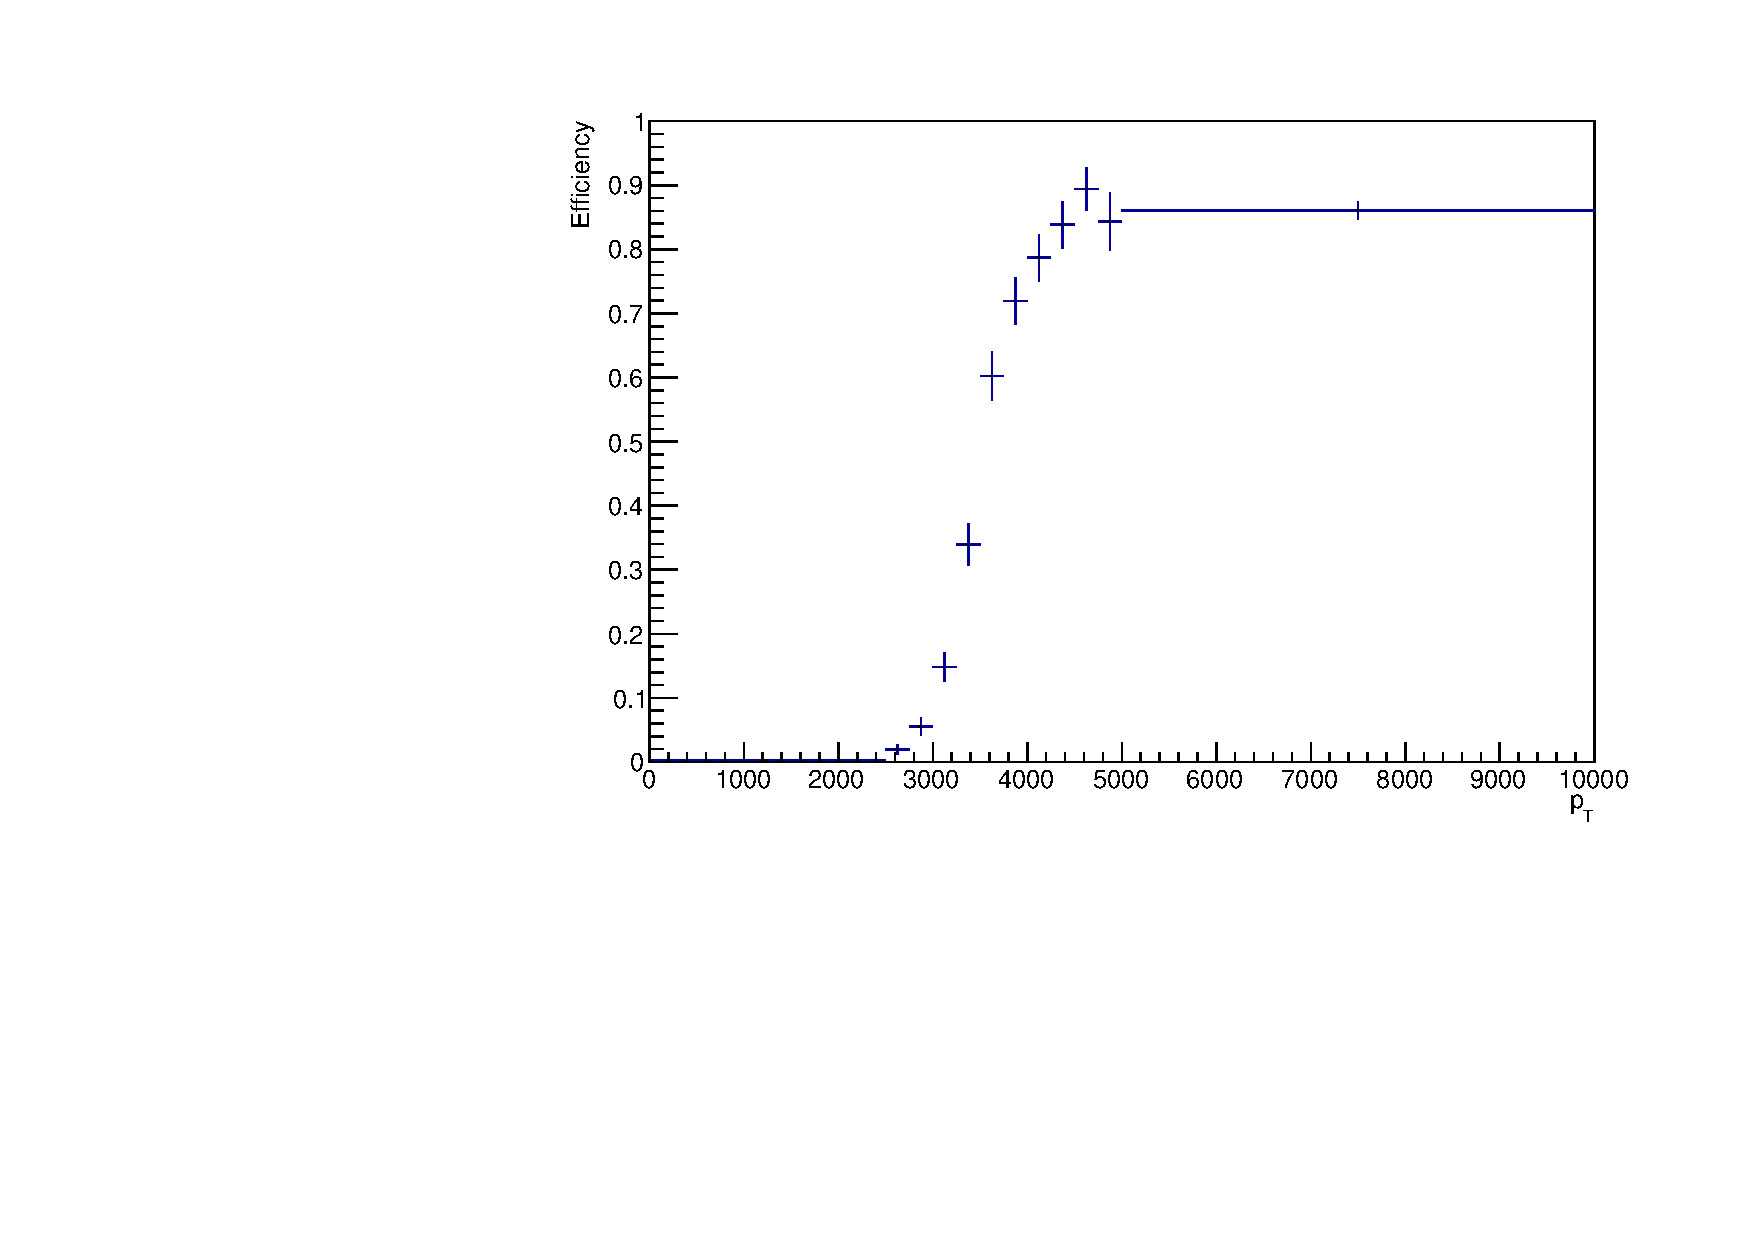
\includegraphics[width=0.48\textwidth]{RKst/figs/l0plots/l0E_Outer.pdf}
\caption{Data-driven L0Electron trigger efficiencies as a function of the transverse momentum
of the electrons for the three ECAL regions.}
\label{sec:L0eff_tables}
\end{figure}

The probability of L0Hadron trigger is calculated for each event as $P_{L0Had} = \varepsilon(\pi) + \varepsilon(K) - \varepsilon(\pi)\varepsilon(K)$.
Similarly the L0Electron trigger probability is $P_{L0Ele} = \varepsilon(e^+) + \varepsilon(e^-) - \varepsilon(e^+)\varepsilon(e^-)$.
Notice that no weight $P_{L0TIS}$ can be defined using the TIS-TOS technique. On the other hand
the probability of TIS trigger is defined to be independent of the signal and thereofre must be the same
in the rare and resonant channels and cancel in their ratio.

Then weights for the three trigger categories are then defined to be exclusive in the following way:

\begin{itemize}
\item L0ElectronTOS: $\varepsilon^{L0E} = P_{L0Ele}$,
\item L0HadronTOS: $\varepsilon^{L0H} = P_{L0Had}\cdot(1 - P_{L0Ele})$, namely the probability that one hadron triggered but none of the electrons,
\item L0TIS: $\varepsilon^{L0I} = (1-P_{L0Had})\cdot(1 - P_{L0Ele})$, namely the probability that neither the hadrons or the electrons in the event triggered.
\end{itemize}

%The total efficiency for each category is then found by using the kinematic distribution from MC events,
%weighted for PID efficiencies, SPD and \Bz $p_T$ as described in \ref{sec:MCweighting}.
As in the PID case, the total efficiency is found averaging over all events of a simulated sample:

\begin{equation}
\varepsilon^{cat} = \frac{1}{N} \sum_i^N \varepsilon^{cat}(p_T^i)
\end{equation}

where $cat$ is a label indicating the trigger category under consideration.


\section{Neural Networks efficiency}
\label{sec:Rkst_mva_eff}

The NN efficiency is again evaluated from fully weighted Monte Carlo samples. 
For the electron channels it is obtained separately for each trigger category,
because the yield is extracted independently for each of the three trigger categories
and therefore these have to be independently corrected.

In order to cross check that this efficiency component is extracted correctly
one can compare the efficiency obtained using $\decay{\Bz}{\jpsi\Kstar}$ events
and rare $\decay{\Bz}{\Kstar \ell^+\ell^-}$ events in the same \qsq region selected
for the resonant case. The ratio between the two should be close to 1 with
small deviations due the fact that the bin width is finite and the events are distributed
differently inside the bin. These ratios are reported in Tab.~\ref{tab:mva_in_jpsibin};
values are not exactly one for the electron channels due to the very large \qsq interval
used to select the resonant channel ([6.0,11.0] \gevgevcccc).

\begin{table}[h!]
\begin{tabular}{|c|c|c|c|c|}
\hline Comp 			&  $\mu\mu$  				& \multicolumn {3}{c|}{$ee$}  \\ \hline
				&   &  L0Electron 	& L0Hadron 	& L0TIS \\ \hline
%rec  & $ 1.0104  \pm  0.0095 $ & \multicolumn{3}{c|}{$ 1.1040  \pm  0.0034 $} \\ 
%\hline
%trg  & $ 1.0113  \pm  0.0055 $ & $ 0.9752  \pm  0.0063 $ & $ 1.0078  \pm  0.0248 $ & $ 0.9766  \pm  0.0113 $ \\ 
mva  & $ 0.9969  \pm  0.0039 $ & $ 0.9771  \pm  0.0023 $ & $ 0.9794  \pm  0.0019 $ & $ 0.9856  \pm  0.0057 $ \\ 
\hline
\end{tabular}
\caption{Ratio $\varepsilon^{\ell\ell} / \varepsilon^{\jpsi}$ where the efficiency for the
rare channel its calculated in the same \qsq rage used to select the resonant channel.}
\label{tab:mva_in_jpsibin}
\end{table}

\clearpage








